%! TEX program = lualatex
\documentclass[12pt]{scrartcl}
% Packages
%\usepackage[margin=1.5in]{geometry}
\usepackage{index}
\usepackage{amsbsy} % Bold math symbols
\makeindex
%\usepackage[utf8]{inputenc}
\usepackage[T1]{fontenc}
\usepackage{tcolorbox}
\tcbuselibrary{theorems}
\tcbuselibrary{skins}
\tcbuselibrary{breakable}
\usepackage{varwidth}
\usepackage{textcomp}
\usepackage{amsmath, amssymb}
\usepackage{esint}
\usepackage{titlesec}
\usepackage{xcolor}
\usepackage{titling}
\usepackage[linktocpage]{hyperref}
\usepackage{pgfplots}
\usepackage{multicol}
\setlength{\columnsep}{2em}
\usepackage{caption}
\usepackage{amsthm}
\usepackage{import}
\usepackage{cancel}
\usepackage{caption}
\usepackage{nicematrix}
\usepackage{mathrsfs}
\usepackage{mathtools}
%\usepackage{parskip}
\usepackage{enumerate}
\usepackage{graphicx}
\usepackage[italian]{babel}
\usepackage{setspace}
\setstretch{1.2}
% To reset footnote numbering each page
\usepackage[perpage]{footmisc}
\usepackage{faktor}
\usepackage{tikz}
\usetikzlibrary{arrows.meta, decorations.pathmorphing, patterns}
\usepackage{tikz-cd}
\definecolor{mastercolor}{HTML}{0c800f}
\definecolor{nred}{HTML}{bf0040}

% Titles 
\title{Appunti di\\ \vspace{.3cm} Geometria e topologia differenziale}
\author{Manuel Deodato}
\date{}




\newtheoremstyle{style}% name of the style to be used
{5pt}% measure of space to leave above the theorem. E.g.: 3pt
{5pt}% measure of space to leave below the theorem. E.g.: 3pt
{\normalfont}% name of font to use in the body of the theorem
%{15pt}% measure of space to indent
{0pt}% measure of space to indent
{\noindent\sffamily\scshape\bfseries}% name of head font
{}% punctuation between head and body
{ }% space after theorem head; " " = normal interword space
{\thmname{#1}\thmnumber{ #2}{\thmnote{ (#3)}.\ }}


\theoremstyle{style}
\newtheorem{esempio}{Esempio}[section]
\newtheorem{definizione}{Definizione}[section]
\newtheorem{prop}{Proposizione}[section]
\newtheorem{teorema}{Teorema}[section]
\newtheorem{lemma}{Lemma}[teorema]
\newtheorem{corollario}{Corollario}[teorema]
\newtheorem{osservazione}{Osservazione}[section]
\newtheorem{notazione}{Notazione}[section]
\newtheorem{esercizio}{Esercizio}[section]





\tcolorboxenvironment{definizione}{blanker,breakable,left=5mm,before skip=10pt,after skip=10pt, borderline west={.5mm}{0pt}{mastercolor}, before upper={\setlength{\parindent}{15pt}}}
\tcolorboxenvironment{lemma}{blanker,breakable,left=5mm,before skip=10pt,after skip=10pt, borderline west={.5mm}{0pt}{mastercolor}, before upper={\setlength{\parindent}{15pt}}}
\tcolorboxenvironment{teorema}{enhanced,blanker,breakable,left=5mm,before skip=10pt,after skip=10pt, borderline west={.5mm}{0pt}{mastercolor}, before upper={\setlength{\parindent}{15pt}}}
\tcolorboxenvironment{corollario}{blanker,breakable,left=5mm,before skip=10pt,after skip=10pt, borderline west={.5mm}{0pt}{mastercolor}, before upper={\setlength{\parindent}{15pt}}}
\tcolorboxenvironment{prop}{blanker,breakable,left=5mm,before skip=10pt,after skip=10pt, borderline west={.5mm}{0pt}{mastercolor}, before upper={\setlength{\parindent}{15pt}}}
\tcolorboxenvironment{esempio}{blanker,breakable,left=5mm,before skip=10pt,after skip=10pt, borderline west={.5mm}{0pt}{mastercolor}, before upper={\setlength{\parindent}{15pt}}}
\tcolorboxenvironment{esercizio}{blanker,breakable,left=5mm,before skip=10pt,after skip=10pt, borderline west={.5mm}{0pt}{mastercolor}, before upper={\setlength{\parindent}{15pt}}}
\tcolorboxenvironment{osservazione}{blanker,breakable,left=5mm,before skip=10pt,after skip=10pt, borderline west={.5mm}{0pt}{mastercolor}, before upper={\setlength{\parindent}{15pt}}}


\newenvironment{svolgimento}{\renewcommand\qedsymbol{$\blacksquare$}\begin{proof}[Svolgimento]}{\end{proof}}




%% Generic box
\newtcolorbox{eqbox}[1][]
{
colback=gray!10,
arc=0pt,
boxrule=0pt,
title=#1
}

 \newenvironment{boxenv}[1][]{
    \begin{eqbox}[#1]
    }{
   \end{eqbox}
}



%Captions
\captionsetup[figure]{font=footnotesize,labelfont=footnotesize}
\captionsetup[table]{font=footnotesize,labelfont=footnotesize}
%Titlesec
\titleformat{\section}
{\fontsize{20}{20}\scshape}
{\normalfont\color{gray}{\fontsize{80}{20}\selectfont\thesection\hspace{.2cm}\color{gray}{\vrule width 1pt}}}
{0.7em}
{}
\titlespacing*{\section}{0pt}{*2}{1cm}
\titlespacing*{\subsection}{0pt}{*5}{.5cm}
\titlespacing*{\subsubsection}{0pt}{*5}{.5cm}

\hypersetup{colorlinks,breaklinks, linkcolor=[RGB]{12,128,15}}

% Personalizza la formattazione della subsection
\titleformat{\subsection}[block]{\centering\fontsize{15}{20}\bfseries}{\color{nred}\normalfont\S\thesubsection}{.5em}{}


% Personalizza la formattazione della subsubsection
\titleformat{\subsubsection}[block]{\centering\fontsize{14}{20}\bfseries}{\color{nred}\normalfont\S\thesubsubsection}{.5em}{}

% Maketitle customization
\renewcommand{\maketitle}{
\begin{center}
{\sffamily
{\fontsize{20}{20}\selectfont\MakeUppercase\thetitle}}

\vspace{0.2in}

{\large\scshape\theauthor}
\end{center}
}

%Evaluate symbol
\DeclareMathOperator{\di}{d\!}
\newcommand*\Eval[3]{\left.#1\right\rvert_{#2}^{#3}}

%%%%%%% Numero delle equazioni in formato a.b
\numberwithin{equation}{subsection}
%%%%%

%%%%%%%%%% Personalizzazione numeri lista
\renewcommand{\theenumi}{(\arabic{enumi})}

%%%% Table of contents

\usepackage[titles]{tocloft}

\renewcommand{\cftdot}{}
\usepackage{titletoc}
%\setcounter{tocdepth}{2}

%%%%%%%%%%%%%%%% Toc style

% Personalizzazione scritta indice


% Font
\renewcommand{\textbf}[1]{\textsf{\bfseries #1}}
\usepackage[osf]{newpxtext}
\usepackage[euler-digits,euler-hat-accent]{eulervm}
\usepackage{fontspec}
\DeclareSymbolFont{operators}{OT1}{EBGaramond-TLF}{m}{n}


\newcommand{\longhookrightarrow}{\lhook\joinrel\longrightarrow}
\begin{document}
\maketitle
\vspace{7cm}
\begin{figure}[h!]
	\centering
	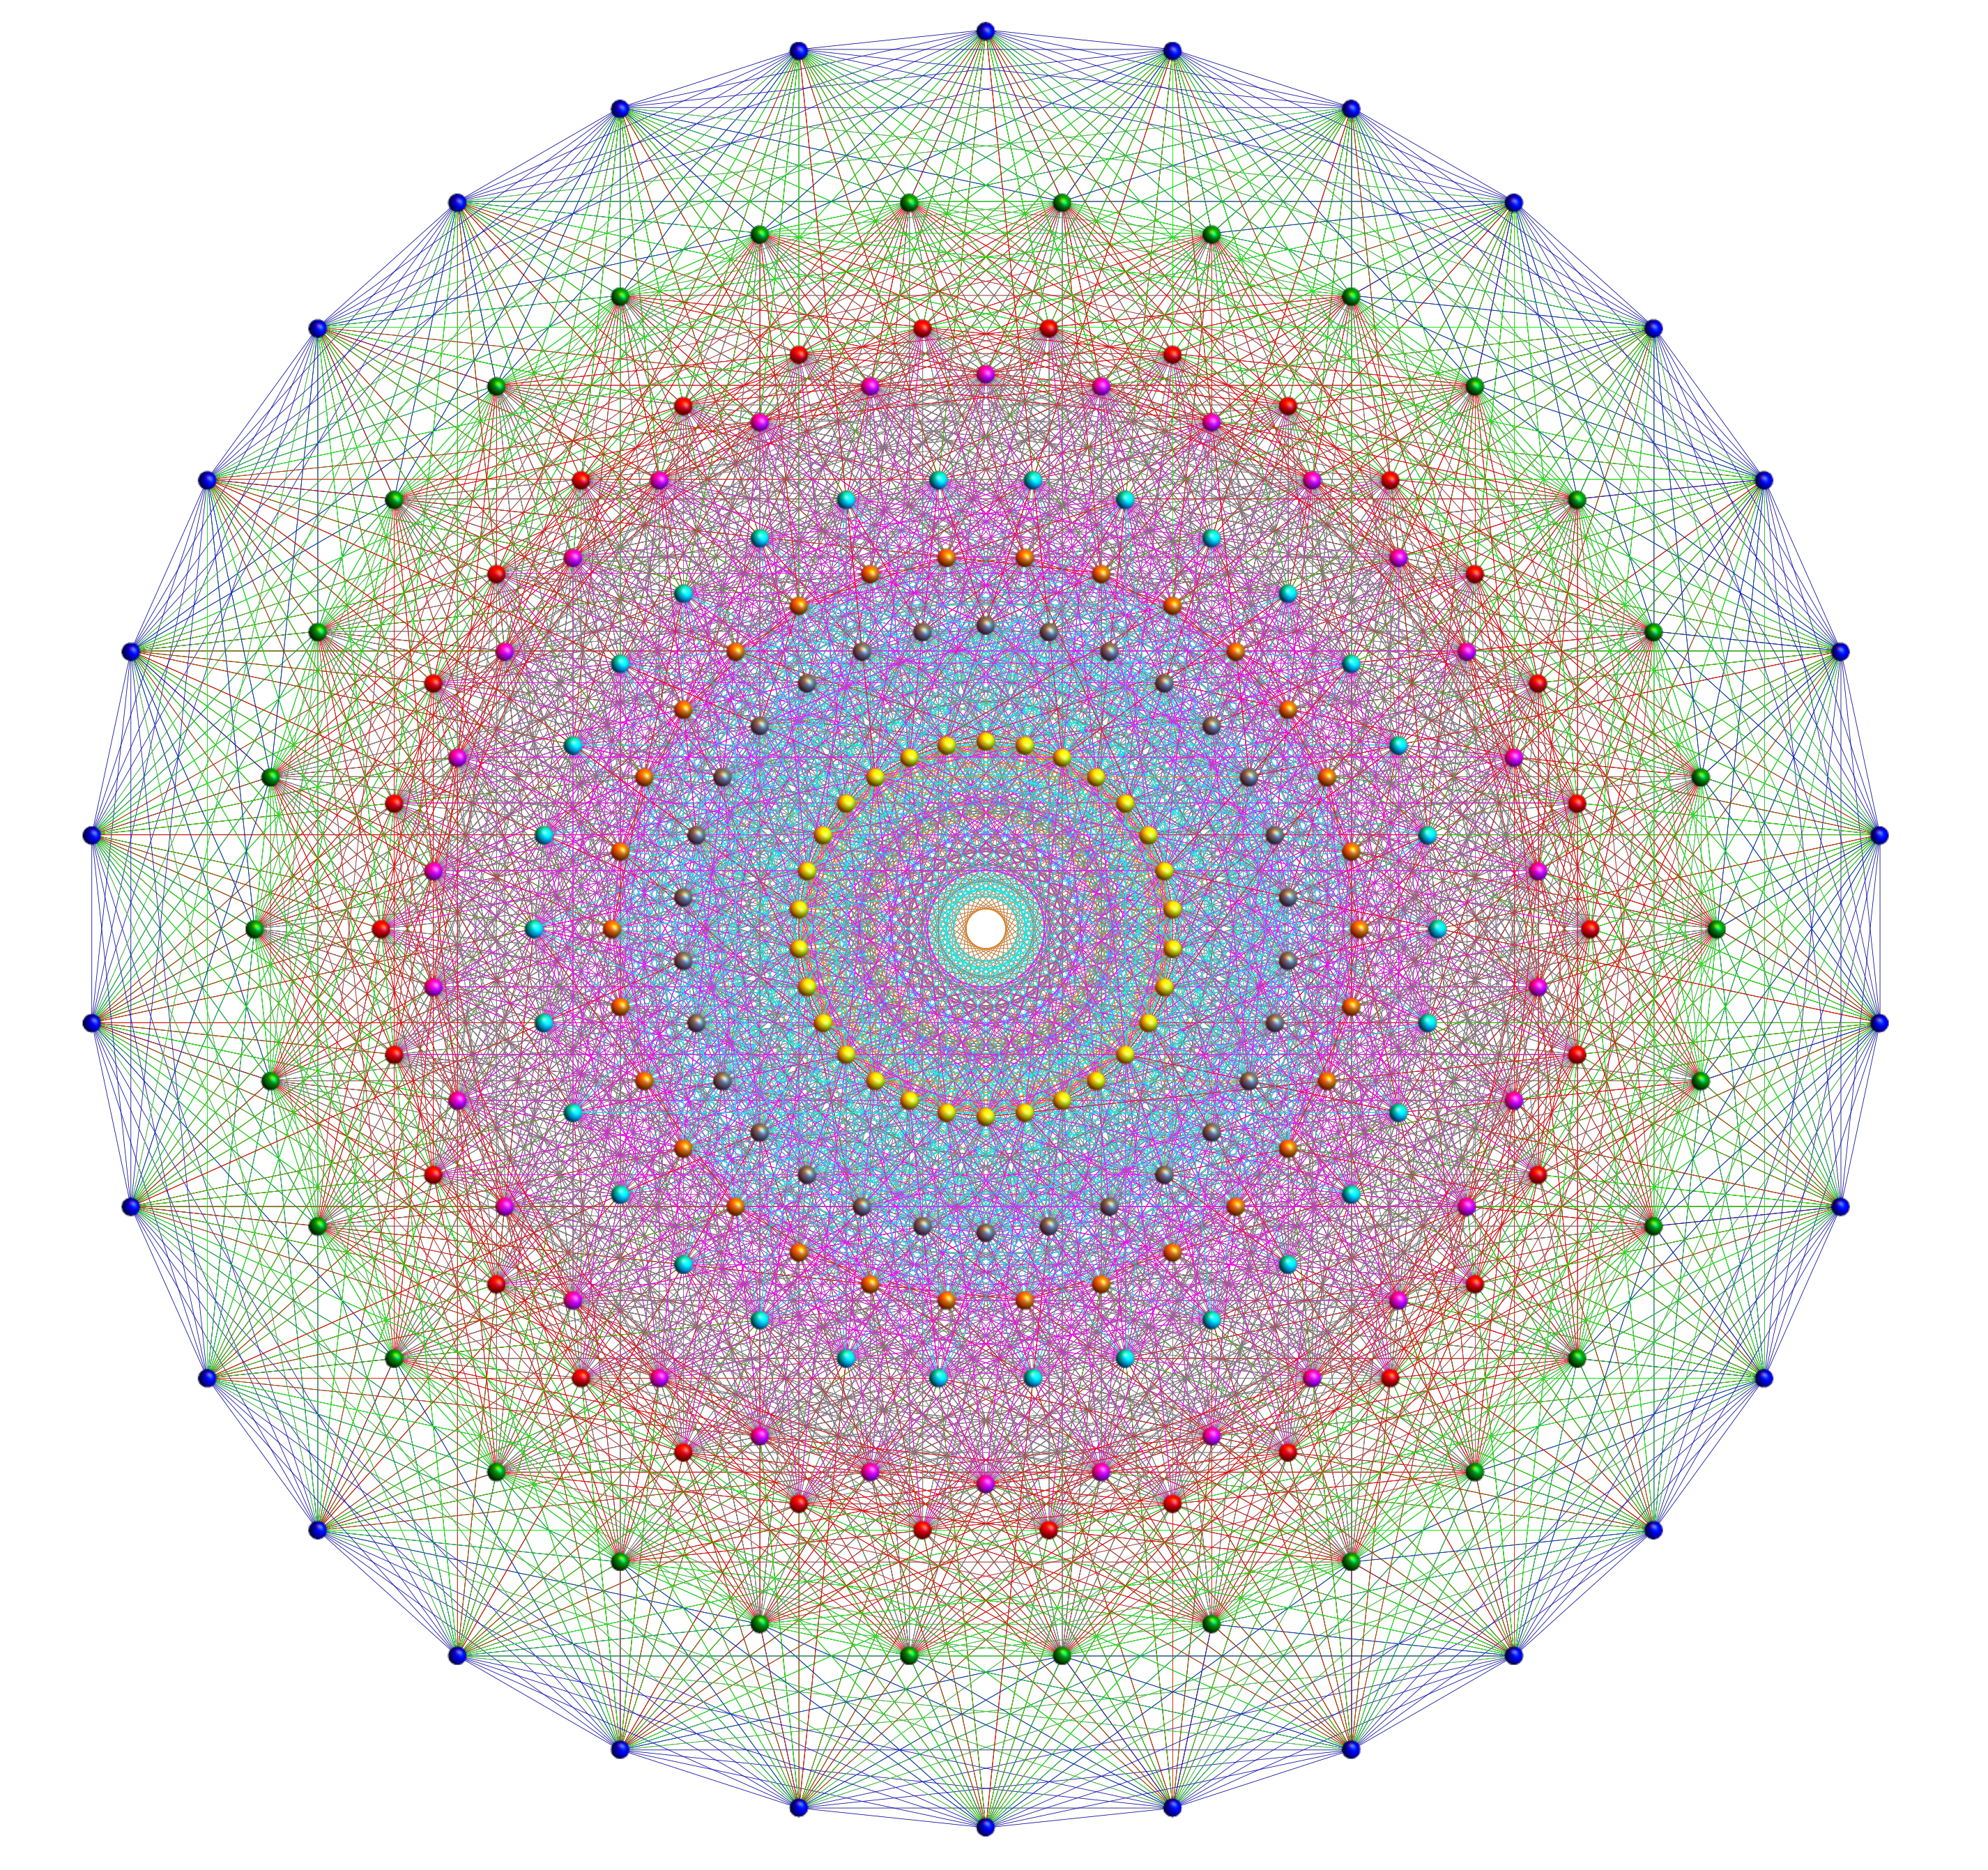
\includegraphics[width=.6\columnwidth]{front.jpg}
\end{figure}

\newpage
\tableofcontents 
\newpage
\section{Teoria delle curve}
\subsection{Introduzione}
\begin{definizione}
	[Curva parametrizzata]
	Una \textit{curva paramtrizzata} \`e un'applicazione $\alpha  : I\subset \mathbb{R} \to \mathbb{R}^3$ di classe $C^\infty(I)$, con $I$ intervallo aperto.
	Data $t\in I$, si pu\`o scrivere in componenti come
	\[
	\alpha (t) = (x(t),y(t),z(t))
	\] 
	con $x,y,z:I\to \mathbb{R}$ tutte di classe $C^\infty(I)$.
\end{definizione}
\begin{osservazione}
La necessit\`a di definire la curva su un aperto, o quantomeno di poter estendere l'intervallo di definizione ad un aperto, deriva dal fatto che, in questo modo, si pu\`o effettivamente parlare di derivata piena anche per gli estremi, potendo trovare, infatti, un aperto che contiene interamente i punti di frontiera dell'intervallo di definizione.
Se non si avesse questa possibilit\`a, nel caso di $\alpha :[a,b] \subset \mathbb{R}\to \mathbb{R}^3$, per esempio, non si potrebbe calcolare la derivata tradizionale in $a$, o $b$, perch\'e si potrebbe solamente calcolare il limite destro o sinistro.
\end{osservazione}
\noindent Si nota che, nel caso in cui $I$ non fosse aperto, si estende l'intervallo di definizione ad $A \supset I$ aperto.

Si parla di \textit{traccia} della curva in riferimento all'immagine che genera dell'intero intervallo: $\operatorname{Tr} \alpha  = \alpha (I)$.
La traccia rappresenta l'unione di ciascun punto di $\alpha (t) \in \mathbb{R}^3, \ \forall t \in I$.
Per \textit{velocit\`a} della curva, invece, si intende la grandezza\footnote{Questa \`e ben definita perch\'e si sta operando in uno spazio vettoriale, con $\alpha (t+h) - \alpha (t)$ giustificata dall'operazione di somma dello spazio e divisione per $h$ data dalla moltiplicazione per uno scalare.}
\begin{equation}
	\alpha '(t) = \lim_{h \to 0} \frac{\alpha (t + h) - \alpha (t)}{h} = \big(x'(t),y'(t),z'(t)\big)
\end{equation}
In realt\`a, questo rappresenta il \textit{vettore velocit\`a}, mentre la velocit\`a vera e propria \`e data dalla sua norma $\left\lVert \alpha' (t) \right\rVert $.
\begin{esempio}
	[Retta parametrizzata]
	Siano $P,Q \in \mathbb{R}^3$, con $P\neq Q$, due punti dello spazio; si definisce, allora, \textit{retta parametrizzata} la curva 
	\[
		\alpha :
		\begin{array}
			{c c c}
			[0,1] &\longrightarrow & \mathbb{R}\\
			t &\longmapsto & P + t(Q-P) = P+t \overrightarrow{PQ}
		\end{array}
	\] 
La sua traccia \`e la retta affine passante per $P$ e $Q$, e ha vettore velocit\`a $\alpha '(t) = \overrightarrow{PQ}$, da cui $\left\lVert \alpha '(t) \right\rVert = \lVert \overrightarrow{PQ} \rVert$, che \`e costante.
\end{esempio}
\begin{esempio}
	[Circonferenza parametrizzata]
Dato $a\in \mathbb{R}$, con $a > 0$, si definisce \textit{circonferenza parametrizzata} come 
\[
\alpha:
	\begin{array}
		{c c c}
		[0,2\pi] &\longrightarrow & \mathbb{R}^3\\
		t &\longmapsto & (a \cos t, a \sin t , 0)
	\end{array}
\] 
il cui vettore velocit\`a \`e dato da $\alpha '(t) = (-a\sin t, a \cos t, 0)$, che non risulta costante, mentre la sua velocit\`a $\left\lVert \alpha ' \right\rVert = a >0$ s\`i.
La traccia corrisponde ad una circonferenza nel piano $z=0$, di centro l'origine e raggio $a$.
\end{esempio}
\subsection{Riparametrizzazione di una curva}
Sia $\alpha : [a,b]\to\mathbb{R}^3$ una curva parametrizzata; una sua \textit{riparametrizzazione} \`e data dalla coppia di mappe $h:[a,b]\to [c,d] \subseteq \mathbb{R}$ e $\beta : [c,d]\to \mathbb{R}^3$ tali che il diagramma
\[
\begin{tikzcd}
	\left[ a,b \right]  & & \mathbb{R}^3\\
	\\
	\left[ c,d \right] 
	\arrow[from=1-1, to=1-3, "\displaystyle \alpha "]
	\arrow[from=1-1,to=3-1,"\displaystyle h"']
	\arrow[from=3-1,to=1-3,"\displaystyle \beta"']
\end{tikzcd}
\] 
commuta, quindi si ha $\beta (h(t)) = \alpha (t)$. 
Perch\'e questo sia verificato, si assume che $h \in C^\infty([a,b])$ e $h'(t) \neq 0, \ \forall t \in [a,b]$; in questo modo, $\exists h^{-1}$ di classe $C^\infty$ tale che $\beta = \alpha \circ h^{-1}$, quindi anche $\beta $ risulta liscia ed \`e verificata la relazione $(\beta \circ h)(t) = \alpha (t)$, con $\operatorname{Tr} \alpha =\operatorname{Tr} \beta $.

Ora si definisce la lunghezza di una curva; se ne giustifica la definizione tramite il seguente ragionamento.
Sia dato $[a,b] \subset \mathbb{R}$ un intervallo e sia $P \in \mathcal{P} ([a,b])$ una sua partizione, tale che $a = t_0 < t_1 < \ldots<t_{k-1} <t_k = b$; allora la lunghezza di una curva $\alpha  : [a,b] \to \mathbb{R}^3$ approssimata a tale partizione \`e data da:
\begin{equation}
	L(\alpha , P) = \sum_{i=0}^{k-1} \left\lVert \alpha (t_{i+1}) - \alpha (t_i) \right\rVert 
\end{equation}
Si nota, dunque, che la lunghezza effettiva della curva coincide con
\begin{equation}
	\sup_{P \in \mathcal{P}([a,b]) } L(\alpha ,P) = \int_{a} ^b \left\lVert \alpha' (u) \right\rVert du
\end{equation}
\begin{definizione}
	[Lunghezza d'arco]
	Sia $\alpha  : [a,b] \subset \mathbb{R}\to \mathbb{R}^3$ una curva; si definisce \textit{lunghezza d'arco} la funzione
	\[
	s :
	\begin{array}
		{c c c}
		[a,b] & \longrightarrow &\mathbb{R}\\
		t & \longmapsto &\displaystyle  \int_{a} ^t \left\lVert \alpha '(u) \right\rVert du
	\end{array}
	\] 
	La lunghezza dell'intera curva $\alpha $ \`e data da $L(\alpha ) = s(b)$.
\end{definizione}
\begin{osservazione}
Si nota che per $\alpha : [0,+\infty) \to \mathbb{R}^3$, con $\alpha  (t) = \big(a \cos t, a \sin t, 0\big)$, valendo $\left\lVert \alpha '(t) \right\rVert = a$, si ha:
\[
s(t) = a \int_{0} ^t du = ta \implies s (2\pi) = 2\pi a
\] 
\end{osservazione}
\noindent Vale la pena chiedersi se $L(\alpha )$ sia indipendente dalla sua parametrizzazione, cio\`e se $L(\alpha ) = L(\beta )$, se $\beta $ \`e una riparametrizzazione di $\alpha $; questo si vede facilmente per conto diretto.
\begin{proof}
	Se $\alpha (t) = \beta (h(t))$, allora $\alpha '(t) = \beta '(h(t)) h'(t)$, quindi
	\[
	L(\alpha ) = \int_{a} ^b \left\lVert \alpha '(t) \right\rVert dt = \int_{a} ^b \lvert h'(t) \rvert \left\lVert \beta '(h(t)) \right\rVert dt
	\] 
	Ora si distinguono due casi: essendo $h'(t)\neq 0, \ \forall t$, si pu\`o avere o $h'(t) <0$, o $h'(t) > 0$. 
	Nel primo caso, si ha $h'(t) < 0$, quindi $\lvert h'(t) \rvert = - h'(t)$, con $h(a) = d$ e $h(b) = c$; nel secondo caso, $\lvert h'(t) \rvert =h'(t)$, con $h(a) = c$ e $h(b) = d$.
	Si trova, per $s = h(t)$, rispettivamente:
	\[
	\begin{cases}
		\displaystyle -\int_{d} ^c h'(t) \left\lVert \beta '(h(t))  \right\rVert dt = \int_{c} ^d \left\lVert \beta '(s) \right\rVert ds = L(\beta )\\
		\\
		\displaystyle \int_{c} ^d h'(t) \left\lVert \beta '(h(t)) \right\rVert dt = \int_{c} ^d \left\lVert \beta '(s) \right\rVert ds = L(\beta )
	\end{cases}
	\] 
In entrambi i casi, dunque, si ottiene $L(\alpha ) = L(\beta )$.	
\end{proof}
\noindent Ora si introduce una particolare riparametrizzazione, talvolta nota col nome di \textit{riparametrizzazione canonica}, o \textit{naturale}; per poterla definire, \`e necessario che $\alpha $ soddisfi la seguente condizione.
\begin{definizione}
	[Curva regolare]
	Una curva parametrizzata $\alpha : I \subset \mathbb{R} \to \mathbb{R}^3$ \`e detta \textit{regolare} se $\alpha '(t) \neq 0, \ \forall t \in I$.
\end{definizione}
\noindent Si considera, quindi, una curva regolare $\alpha :[a,b] \to \mathbb{R}^3$; visto che $s(t) = \int_{a} ^t \left\lVert \alpha '(u) \right\rVert du$, allora $s'(t) = \left\lVert \alpha '(t) \right\rVert >0$.
Si pu\`o pensare alla lunghezza d'arco come $s : [a,b] \to [0, L(\alpha )]$, che, essendo monotona perch\'e si \`e appena osservato che $s'(t) > 0$, allora ha anche inversa $t : [0,L(\alpha )]\to [a,b]$.
\`E, quindi, possibile definire la funzione 
\begin{equation}
	\beta = \alpha \circ t : [0,L(\alpha )]\to \mathbb{R}^3
\end{equation}
tale che $\operatorname{Tr} (\beta )=\operatorname{Tr} (\alpha ) $ e $\beta (s) = \alpha (t(s))$, per cui
\[
\beta '(s) = \alpha '(t(s)) t'(s) = \frac{\alpha '(t(s))}{s'(t(s))} = \frac{\alpha '(t(s))}{\left\lVert \alpha '(t) \right\rVert }
\] 
per cui $\left\lVert \beta '(s) \right\rVert =1$.
\begin{definizione}
	[Curva p.l.a.]
	Se $\alpha :I\to\mathbb{R}^3$ \`e una curva tale che $\left\lVert \alpha '(t)\right\rVert = 1 , \ \forall t \in I$, allora si dice che \`e \textit{parametrizzata tramite lunghezza d'arco}, o pla.
\end{definizione}
\begin{osservazione}
In base a quanto detto prima, ogni curva regolare \`e \textit{riparametrizzabile tramite lunghezza d'arco}.
\end{osservazione}
\begin{osservazione}
	[Non unicit\`a della versione pla]
	Data una curva regolare $\alpha  : I \to \mathbb{R}^3$, la riparametrizzazione tramite lunghezza d'arco non \`e univoca ma dipende dall'estremo inferiore di integrazione della lunghezza d'arco $s(t)$; se, infatti, $a,b \in I$ con $a < b$:
	\[
	s_a (t) = \int_{a} ^t \left\lVert \alpha '(u) \right\rVert du \hspace{1cm}s_b (t) \int_{b} ^t \left\lVert \alpha '(u) \right\rVert du
	\] 
	Le due, per\`o, differiscono solo per una costante perch\'e
	\[
	s_a(t) = \int_{a} ^b \left\lVert \alpha '(u) \right\rVert du + \int_{b} ^t \left\lVert \alpha '(u) \right\rVert du = \text{cost.} + s_b(t)
	\] 
	Questa differenza per una costante non influir\`a sulla trattazione del riferimento di Frenet perch\'e si lavora con derivate e la costante sparisce.
\end{osservazione}
\begin{esempio}
	[Elica]
Sia $a > 0$; allora la mappa
\[
\varphi :
\begin{array}
	{c c c}
	\mathbb{R}^2 & \longrightarrow & \mathbb{R}^3\\
	(u,z) &\longmapsto & (a \cos u , a \sin u , z)
\end{array}
\] 
definisce un cilindro di raggio $a$ attorno all'asse $z$.
Preso $b > 0$ e presi i punti $\left\{ (t,bt) \right\} _{t \in \mathbb{R}} $, relativi ad una retta passante per l'origine, aperto, si pu\`o definire la curva 
\[
\alpha (t) = \varphi (t,bt) = (a \cos t , a \sin t , bt)
\] 
che descrive un'\textit{elica destrorsa}, visto che si \`e preso $b>0$\footnote{Fosse stato $b<0$, sarebbe stata un'\textit{elica sinistrorsa}.}, di raggio $a$ e passo $b$.
Si nota che
\[
\alpha '(t) = (-a \sin t, a \cos t , b) \implies \left\lVert \alpha '(t) \right\rVert =\sqrt{a^2 + b^2} > 0, \ \forall t \in \mathbb{R}
\] 
da cui $\alpha $ \`e regolare. 
Restringendola a $[0,+\infty)$, cio\`e considerando $\alpha : [0,+\infty) \to \mathbb{R}^{3} $, si ha:
\[
	s(t) = \int_{0} ^t \sqrt{a^2 + b^2 }  du = t(s) \sqrt{a^2 + b^2} \implies t(s) = \frac{s}{\sqrt{a^2 +b^2}}
\] 
quindi:
\[
\begin{split}
		 \beta (s) &= \alpha (t(s)) = \alpha  \left(\frac{s}{\sqrt{a^2 + b^2} }\right) \\
	&= \left(a \cos \left(\frac{s}{\sqrt{a^2+b^2} }\right) , a\sin \left(\frac{s}{\sqrt{a^2 + b^2} }\right),\frac{bs}{\sqrt{a^2 + b^2} } \right)
	\end{split} 
\] 
con $\beta $ pla e, conseguentemente, $\beta (\mathbb{R}) = \operatorname{Tr} (\beta ) = \operatorname{Tr} (\alpha ) = \alpha (\mathbb{R})$.
\end{esempio}
\begin{esempio}
	[Ellisse]
	Siano $a,b \in \mathbb{R}\setminus\left\{ 0 \right\} $ e sia 
	\[
	\mathcal{E} _{a,b} = \left\{ (x,y,0) \in \mathbb{R}^3  \ \bigg\lvert \ \frac{x^2}{a^2} + \frac{y^2}{b^2} = 1\right\} \subset \mathbb{R}^3
	\] 
	Si vuole definire una curva $\alpha $ tale che $\operatorname{Tr} \alpha = \mathcal{E} _{a,b} $
\end{esempio}
	\begin{svolgimento}
		Si nota che $(x /  a , y / b) \in S^1$, cio\`e
	\[
	\frac{x}{a} = \cos t \hspace{1cm}\frac{y}{b} = \sin t
	\] 
	con $S^1$ circonferenza unitaria e $t\in [0,2\pi)$.
	Sia, allora
	\[
\alpha :
	\begin{array}
		{c c c}
		[0,2\pi) &\longrightarrow & \mathbb{R}^3\\
		t & \longmapsto & (a \cos t , b \sin t, 0)
	\end{array}
	\] 
 e si vede che $\operatorname{Tr} \alpha  = \mathcal{E} _{a,b} $.

	\end{svolgimento}
\begin{esempio}
Sia 
\[
\mathcal{C}  = \left\{ (x,y,0) \in \mathbb{R}^3  \mid y^2 = x^3 \right\}  \subset \mathbb{R}^3
\] 
Si vuole costruire $\alpha $ tale che $\operatorname{Tr}\alpha  = \mathcal{C} $.
\end{esempio}
\begin{svolgimento}
	Se si considera la secante $y = tx$, allora $t^2 x^2 = x^3$, ossia $x= t^2$ e $y = t^3$.
	Ne segue che la curva che soddisfa la richiesta \`e $\alpha (t) = (t^2 , t^3,0)$.
\end{svolgimento}
\begin{esempio}
Sia 
\[
\mathcal{C}  = \left\{ (x,y,0)  \mid y^2 = x^3 + x^2 \right\} \subset \mathbb{R}^3
\] 
Si vuole costruire una curva $\alpha $ tale che $\operatorname{Tr} \alpha  = \mathcal{C} $.
\end{esempio}
\begin{svolgimento}
	Si considera, come prima, $y=tx $, da cui $x^3 + x^2(1-t^2) = 0$, e si vede che $x = t^2 - 1$ e $y=t^3 -t$, quindi $\alpha (t) = (t^2 - 1, t^3-t,0)$.
\end{svolgimento}
\noindent Per quanto in linea teorica se $\alpha $ \`e una curva regolare, allora si pu\`o riparametrizzare tramite lunghezza d'arco, questo non \`e praticamente fattibile in ogni singolo caso; se, per esempio, si considera $\alpha (t) = (t,t^2,t^3)$, si ha $\alpha '(t) = (1,2t,3t^2)$, che, dunque, \`e regolare, ma data
\[
s(t) = \int_{0} ^t \sqrt{1 + 4u^2 + 9u^4} du
\] 
non si \`e in grado di trovare un'espressione per $t(s)$ perch\'e la primitiva di $s$ non \`e scrivibile in termini di funzioni elementari.
\subsection{Riferimento ed equazioni di Frenet}
\begin{definizione}
	[Versore tangente]
	Data una curva riparametrizzabile $\alpha :I \to \mathbb{R}^3$ e la sua riparametrizzazione tramite lunghezza d'arco $\beta (s)$, si definisce il \textit{versore tangente} ad $\alpha $ come $T(s) = \beta '(s)$.
\end{definizione}
\begin{definizione}
	[Curvatura]
	Data una curva pla $\beta :I\to \mathbb{R}^3$ e il suo versore tangente $T(s)$, allora se ne definisce la \textit{curvatura} come
	\[
	k (s) = \left\lVert T'(s) \right\rVert 
	\] 
\end{definizione}
\noindent Ora si ricavano il riferimento di Frenet e le equazioni di Frenet.
Per poter definire il riferimento di Frenet e ricavare, conseguentemente, le equazioni di Frenet, \`e necessario imporre ulteriori condizioni sulle curve in esame; la condizione operativa necessaria \`e la seguente.
\begin{definizione}
	[Curva di Frenet]
	Una curva regolare $\alpha:[a,b]\to\mathbb{R}^3 $ \`e detta \textit{di Frenet} se la sua pla $\beta = \alpha  \circ t:[0,L(\alpha )]\to \mathbb{R}^3$ \`e tale che $k(s) >0, \ \forall s \in [0,L(\alpha )]$.
\end{definizione}
\begin{lemma}\label{lemdif}
	Se $f, g : I \to \mathbb{R}^{3} $ sono due mappe, allora 
	\[
	\left(f(t)\cdot g(t)\right) ' = f'(t) \cdot g(t) + f(t) \cdot g'(t)
	\] 
\end{lemma}
	\begin{proof}
		Si ha
		\[
		f(t) \cdot g(t) = \sum_{i=1}^{3} f_i(t) g_i(t)
		\] 
	quindi
	\[
	\left(f(t)\cdot g(t)\right) ' = \sum_{i=1}^{3} \left[ f_i'(t)g_i(t) + f_i(t) g_i'(t) \right] 
	\] 
	\end{proof}
\noindent Data $\alpha : I \to \mathbb{R}^3$ una curva di Frenet e $T(s) = \beta '(s)	$ il suo versore normale, con $\beta $ versione pla di $\alpha $, si nota che $T'(s)$ non \`e, in generale un versore e 
\[
1 = \left\lVert T(s) \right\rVert ^2 = T(s) \cdot T(s) \implies \left[ T(s) \cdot T(s) \right] ' = 2T'(s) \cdot T(s) = 0 \implies T'(s) \perp T(s) 
\] 
Avendo assunto $\alpha $ di Frenet, significa che $k_\alpha  (s) \neq 0$, quindi $T'(s)$ \`e normalizzabile e si ottiene un versore ortogonale a $T(s)$.
Usando questo versore e $T(s)$, tramite il prodotto vettore, se ne pu\`o definire un terzo; allora si ha la seguente definizione.
\begin{definizione}
	[Versori normale e binormale]
	Dato $T(s)$ versore tangente di una curva di Frenet $\alpha : I \to \mathbb{R}^3$, si definiscono $N(s) = T'(s) / \left\lVert T'(s) \right\rVert $ \textit{versore normale principale} e $B(s) = T(s) \times N(s)$ \textit{versore binormale}.
\end{definizione}
\noindent Evidentemente, si ha $\left\lVert N(s) \right\rVert =\left\lVert B(s) \right\rVert  = 1 $ e $T(s) \cdot N(s) = T(s) \cdot B(s) = N(s) \cdot B(s) =  0 $.
Ne segue che $\big(T(s),N(s),B(s)\big), \ \forall s \in I$ forma una base ortonormale di $\mathbb{R}^3$, nota col nome di \textbf{riferimento di Frenet}.
Per definizione di $N(s)$, si ottiene la \textbf{I equazione di Frenet}:
\begin{boxenv}[]
\begin{equation}
	T'(s) = k(s) N(s)
\end{equation}
\end{boxenv}
\noindent Si nota che, essendo un versore, si ha $N(s) \cdot N(s) = 1$, quindi $N'(s) \cdot N(s) = 0$ (per lo stesso ragionamento fatto per $T(s)$), dunque $N'(s) \in \langle T(s) , B(s) \rangle$; inoltre, essendo $T(s)\cdot N(s) = 0$, si ha 
\[
	T'(s) \cdot N(s) +T(s)\cdot  N'(s)=k(s) \underbracket{N(s) \cdot N(s)}_{=1}  +T(s)\cdot  N'(s) = 0 
\] 
perci\`o si trova $ \tau (s)$ tale per cui 
\begin{boxenv}[]
\begin{equation}
	N'(s) = -k(s)  T(s) + \tau (s)  B(s)
\end{equation}
\end{boxenv}
\noindent Questa \`e nota come \textbf{II equazione di Frenet}.
\begin{definizione}
	[Torsione]
	Data una curva regolare $\alpha :I\to\mathbb{R}^3$ e $\beta $ la sua pla, si definisce $\tau (s)$ come la \textit{torsione} di $\beta $ nel punto $s$.
\end{definizione}
\noindent Ripetendo lo stesso ragionamento, si ha $B(s) \cdot B(s) = 1 \Rightarrow B'(s) \cdot B(s) = 0$, da cui $B'(s) \in \langle T(s),N(s) \rangle$ e, essendo $N(s) \cdot B(s) = 0$, dalla derivata di $T(s) \cdot B(s) = 0$, si ha
\[
	T'(s) \cdot B(s) + T(s) \cdot B'(s) = k(s) \underbracket{N(s) \cdot B(s)}_{=0}  + T(s) \cdot B'(s) = 0
\] 
quindi $B'(s) \in \langle N(s) \rangle$.
Usando $T(s) \cdot B(s) = 0 $ e derivando $N(s) \cdot B(s) = 0$, si ottiene
\[
	\begin{split}
		N'(s) \cdot B(s) + N(s) \cdot B'(s) &= (- k(s) T(s) + \tau (s) B(s) )\cdot B(s) + N(s) \cdot B'(s) \\
		&= \tau (s) \underbracket{B(s)\cdot B(s)}_{=1}  + N(s)\cdot B'(s) = 0 
	\end{split}
\] 
cio\`e
\begin{boxenv}[]
\begin{equation}
	B'(s) = - \tau (s) N(s)
\end{equation}
\end{boxenv}
\noindent che \`e nota come \textbf{III equazione di Frenet}.
Ricapitolando, le equazioni di Frenet stabiliscono delle relazioni tra le derivate dei versori ortonormali del riferimento di Frenet e i versori stessi e sono:
\begin{boxenv}[]
\begin{equation}
	\begin{cases}
		T'(s) = k(s) N(s)\\
		N'(s) = - k(s) T(s) + \tau (s) B(s)\\
		B'(s)=-\tau (s) N(s)
	\end{cases}
\end{equation}
\end{boxenv}
\noindent Ora si applicano i concetti visti alle curve studiate nella sezione precedente.
\begin{esempio}
	Sia $\alpha (t) = P + t \overrightarrow{PQ}$ una curva parametrizzata (con $P,Q \in \mathbb{R}^3$ e $P\neq Q$). 
	Si ha $\alpha '(t) = \overrightarrow{PQ}$, quindi la curva \`e regolare, quindi se ne pu\`o trovare una pla:
	\[
		s(t) = \int_{a} ^t \lVert \overrightarrow{PQ} \rVert du= t \lVert \overrightarrow{PQ} \rVert \implies t = \frac{s}{\lVert \overrightarrow{PQ} \rVert }
	\] 
	quindi si ha $\beta (s) = P + s \frac{\overrightarrow{PQ}}{\lVert \overrightarrow{PQ} \rVert }$. 
	Allora il versore tangente \`e dato da 
	\[
	T(s) = \beta '(s) = \frac{\overrightarrow{PQ}}{\lVert \overrightarrow{PQ} \rVert } \implies T'(s) = 0 
	\] 
	perci\`o $k(s) = 0$ e, quindi, $\alpha $ non \`e una curva di Frenet perch\'e non ha curvatura positiva.
\end{esempio}
\begin{esempio}
Per $a>0$, sia $\alpha (t) = (a \cos t, a \sin t, 0)$ una circonferenza parametrizzata di raggio $a$.
Evidentemente, si pu\`o vedere come un caso particolare di elica parametrizzata per $b=0$, quindi si pu\`o fare uso del risultato trovato in precedenza:
\[
	\begin{split}
		&\beta (s) = \left(a \cos \left(\frac{s}{a}\right) , a\sin \left(\frac{s}{a}\right),0 \right)\implies T(s) = \left(- \sin \frac{s}{a}, \cos \frac{s}{a},0 \right) \\
		&\Rightarrow T'(s) = \underbracket{\frac{1}{a}}_{k(s)}  \underbracket{\left(-\cos \frac{s}{a},- \sin \frac{s}{a},0\right) }_{N(s)} 
	\end{split}
\] 
Si conclude che $N(s)\perp z$ e punta proprio verso $z$; inoltre, la circonferenza parametrizzata \`e una curva di Frenet perch\'e ha curvatura positiva, essendo $1 / a > 0 $ perch\'e $a > 0 $ per assunzione.
Infine:
\[
	\begin{split}
		&B(s) = \begin{pmatrix} -\sin s / a \\ \cos s / a \\ 0  \end{pmatrix} \times \begin{pmatrix} - \cos s / a\\ - \sin s / a \\ 0  \end{pmatrix} = \begin{pmatrix} 0 \\0 \\ 1 \end{pmatrix} \\
		&\Rightarrow -\tau (s) N(s) = B'(s) = 0 \implies \tau (s) = 0 
	\end{split}
\] 
\end{esempio}
\begin{esempio}
Si considera l'elica parametrizzata $\alpha = (a\cos t , a \sin t, bt)$, con raggio $a\in \mathbb{R}^{>0} $ e passo $b \in \mathbb{R}$.
La sua pla \`e gi\`a stata ricava; dato $c = \sqrt{a^2 + b^2} $, si ottiene:
\[
	\beta (s)= \left(a \cos \left(\frac{s}{\sqrt{c} }\right) , a\sin \left(\frac{s}{\sqrt{c} }\right),\frac{b}{\sqrt{c} } s\right)
\] 
da cui
\[
	T(s) = \frac{1}{c}\left(-a \sin \frac{s}{c}, a \cos \frac{s}{c}, b\right) \implies T'(s) = \underbracket{\frac{a}{c^2}}_{k(s)} \underbracket{\left(-\cos \frac{s}{c},- \sin \frac{s}{c},0\right) }_{N(s)} 
\] 
quindi, come nel caso della circonferenza, $N(s)\perp z$ e punta verso di esso.
Si ha:
\[
B(s) = \frac{1}{c} \begin{pmatrix} - a \sin s / c\\ a \cos s / c\\ b  \end{pmatrix} \times \begin{pmatrix} - \cos s / c \\ - \sin s / c \\ 0  \end{pmatrix} = \frac{1}{c} \begin{pmatrix} b \sin s / c \\ - b \cos  s / c \\ a  \end{pmatrix} 
\] 
Inoltre:
\[
	N'(s) = - k(s) T(s) +\tau (s) B(s) \implies \tau (s) = N'(s) \cdot B(s) =  \frac{b}{c^2}
\] 
Da questo, si vede che
\begin{itemize}
	\item se $b>0$, allora l'elica \`e destrorsa e $\tau (s) >0$,
	\item se $b<0$, allora l'elica \`e sinistrorsa e $\tau (s) < 0 $,
	\item se $b=0$, si ha una circonferenza e $\tau (s) = 0 $, con $k(s) = 1 / a$.
\end{itemize}
Fissando $a$, si nota che, per $b \to \pm \infty$, si ha $\tau (s) \to 0$ e $k(s) = a / (a^2 + b^2) \to 0 $.
\end{esempio}
\begin{prop}
	Sia $\alpha  : I \to \mathbb{R}^3$ una curva regolare; allora $k_\alpha = 0 \iff \alpha (I)$ \`e contenuta in una retta.
\end{prop}
	\begin{proof}
		Si divide la dimostrazione nelle due implicazioni.
		\begin{itemize}
			\item ($\Leftarrow$) Se $\alpha (I) \subseteq P+ \langle v \rangle$, per $v$ versore generico, si considera la sua versione pla $\alpha (I) = \beta (J) \subseteq P+\langle v \rangle$; allora $\beta = P + f(s) v$ e $\beta '=f'(s) v$, con $f'(s)=\pm 1$ perch\'e $\left\lVert \beta ' \right\rVert = 1$. 
				Ne segue che:
				\[
				T(s) = \beta '(s) = f'(s) v = \pm v \implies T'(s) = 0 \implies k_\alpha(s) = 0 
				\] 
			\item ($\Rightarrow $) Sia $\left\lVert T'(s) \right\rVert = k_\alpha (s) = 0 $, quindi $T(s) = \beta '(s) = v $, per qualche $v \in \mathbb{R}^3$.
				Allora si deve avere $\beta (s) =  \beta (0)+ s v \in \beta (0) +\langle v \rangle$.
		\end{itemize}
	\end{proof}
\begin{esercizio}
Sia $\beta :I \to \mathbb{R}^3$ una curva pla tale che
\[
\beta (I) \subseteq S_r^2(P) = \left\{ x \in \mathbb{R}^3 \ \big\lvert\ \left\lVert x- P \right\rVert = r\right\} 
\] 
Mostrare che $\beta  $ \`e di Frenet.
\end{esercizio}
\begin{svolgimento}
	Se $\beta (I) \subseteq S_r^2(P)$, allora $\left\lVert \beta (s) - P \right\rVert ^2 = r^2$; derivando due volte rispetto a $s$, si ottiene:
	\[
		\begin{split}
			&\frac{d }{d s}\left[  T(s) \cdot (\beta (s) - P )  \right] = 0 \implies T'(s) \cdot (\beta (s) - P) + T(s) \cdot T(s) = 0 \\
			&\Rightarrow T'(s) \cdot (\beta (s) - P) = -1 \implies k(s) \left[ N(s) \cdot (\beta (s) - P) \right] = - 1
		\end{split}
	\] 
	Quindi $k(s) \neq 0$ e, pertanto $\beta $ \`e di Frenet.
\end{svolgimento}
\begin{prop}
	Sia $\alpha  : I \to \mathbb{R}^3$ una curva di Frenet; allora $\tau _\alpha = 0 \iff \alpha (I)$ \`e contenuta in un piano.
\end{prop}
	\begin{proof}
		Si divide la dimostrazione nelle due implicazioni.
		\begin{itemize}
			\item ($\Rightarrow $) Si assume, senza perdita di generalit\`a, che $\alpha $ sia pla\footnote{Altrimenti, $\alpha $ ammette una versione pla perch\'e \`e una curva di Frenet.}.
				Allora 
				\[
				\tau _\alpha  = 0 \implies B'_\alpha (s) = - \tau _\alpha (s) N_\alpha (s) = 0 
				\] 
				quindi $B_\alpha $ \`e costante; sia $B_\alpha (s) = B_0$, per qualche $B_0\in \mathbb{R}^3$ tale che $\left\lVert B_0 \right\rVert =1$.
				Ne segue, allora, che
				\[
				T(s) \cdot B_0 = \alpha '(s) \cdot B_0\implies (\alpha (s) \cdot B_0)' = 0
				\] 
				quindi $\alpha (s)\cdot B_0 = c \in \mathbb{R}$, dunque $\alpha (I) \subseteq \left\{ x \in \mathbb{R}^3  \mid x\cdot B_0 = c \right\} $.
			\item ($\Leftarrow$) Sia $\alpha (I) \subseteq \left\{ x \in \mathbb{R}^3  \mid x\cdot B_0 =c  \right\} $, per qualche $B_0 \in \mathbb{R}^3$ tale che $\left\lVert B_0  \right\rVert  = 1$ e $c \in \mathbb{R}$; allora $\forall s, \ \alpha (s) \cdot B_0 = c$.
				Ne segue che
				\[
				T(s) \cdot B_0 = 0 \implies k(s) (N(s) \cdot B_0) = 0 \implies N(s) \cdot B_0 = 0
				\] 
				dove la seconda implicazione \`e giustificata dal fatto che $\alpha $ \`e di Frenet, quindi $k(s) > 0 $.
				Visto che $B_\alpha (s) = T(s) \times N(s)$, considerando (continuare \ldots).
		\end{itemize}
	\end{proof}
\begin{prop}
	Sia $\alpha : I \to \mathbb{R}^3$ una curva di Frenet; se $\tau _\alpha  = 0$, allora $k_\alpha $ \`e costante $\iff \alpha (I)$ \`e contenuta in una circonferenza.
\end{prop}
\begin{proof}
{\color{nred} Da scrivere\ldots}
\end{proof}
\begin{prop}
	Sia $\alpha : I \to \mathbb{R}^3$ una curva regolare; se $\alpha (I) \subseteq \mathbb{S}_R(P) = \left\{ x \in \mathbb{R}^3  \mid \left\lVert x - P \right\rVert = R \right\} $, allora $\alpha $ \`e di Frenet e $k_\alpha \ge 1 / R > 0$.
\end{prop}
\begin{proof}
	Sia $\beta $ la versione pla di $\alpha $. Assumendo che $\operatorname{Tr} (\beta ) \subseteq \mathbb{S}_R(P)$, si ha:
	\[
		(\beta (s) - P) \cdot (\beta (s) - P) = \left\lVert \beta (s) - P \right\rVert ^2 = R^2
	\] 
	Derivando questa relazione, si ha:
	\[
	\beta '(s) \cdot (\beta (s) - P) = 0
	\] 
	Derivando nuovamente:
	\[
		T'(s) \cdot (\beta (s)-P) + \underbracket{\beta '(s) \cdot \beta '(s)}_{=1}  = 0 
	\] 
	Passando alla norma, si vede che:
	\[
	1=\left\lVert T'(s) \cdot (\beta (s) - P) \right\rVert \le \left\lVert T'(s) \right\rVert \left\lVert \beta (s) - P \right\rVert = k_\alpha (s) R
\] 
	da cui $k_\alpha (s) \ge 1 / R > 0$, quindi $\alpha $ \`e di Frenet.
\end{proof}
\subsection{Riferimento di Frenet senza lunghezza d'arco}
Come accennato, la possibilit\`a di ottenere la versione pla di una curva regolare, anche se ammissibile in teoria, non sempre \`e concreta in pratica.

Sia, allora, $\alpha : I \to \mathbb{R}^3$ una curva regolare; per definzione
\[
	\beta (s(t))= \alpha (t) \implies \beta '(s(t)) s'(t) = \beta '(s(t)) \left\lVert \alpha '(t) \right\rVert = \alpha '(t)
\] 
da cui si ottiene la relazione
\begin{boxenv}[]
\[
	T(s(t)) = \frac{\alpha '(t)}{\left\lVert \alpha '(t) \right\rVert }
\] 
\end{boxenv}
\noindent Dalla relazione precedente, sostituendo $\beta '(s(t)) = T(s(t))$, si ottiene
\begin{equation}
	s'(t) T(s(t)) = \alpha '(t)
\end{equation}
e, derivando:
\begin{equation}\label{e1}
s'' (t) T(s(t)) + s'^2(t) T'(s(t)) = \alpha ''(t)
\end{equation}
A questo punto, si vede che, facendo il prodotto vettore $\alpha ' \times \alpha ''$, il termine $T' \times T' = 0$, quindi:
\begin{equation}\label{e2}
	\alpha ' \times \alpha '' = s'^3 T\times T'
\end{equation}
Si nota che, essendo $T ' \perp T $ e $\left\lVert T \right\rVert = 1$, si ha $\left\lVert T ' \times T \right\rVert = \left\lVert T' \right\rVert = k$, perci\`o
\begin{boxenv}[]
\[
k = \frac{\left\lVert \alpha '\times \alpha '' \right\rVert }{s'^3}= \frac{\left\lVert \alpha ' \times \alpha ''\right\rVert }{\left\lVert \alpha '\right\rVert ^3}
\] 
\end{boxenv}
\noindent Per continuare, si assume che $\alpha $ sia una curva di Frenet; allora, usando la I equazione di Frenet, si ottiene
\[
	s'^3 k \underbracket{T \times N }_{=B} = \alpha ' \times \alpha ''
\] 
da cui si ottiene
\begin{boxenv}[]
\[
B=\frac{\alpha '\times \alpha ''}{\left\lVert \alpha ' \right\rVert ^3 k} =\frac{\alpha ' \times \alpha ''}{\left\lVert \alpha ' \times \alpha '' \right\rVert }
\] 
\end{boxenv}
\noindent Da questo, si ricava 
\begin{boxenv}[]
\[
N = B \times T = \frac{\alpha ' \times \alpha '' \times \alpha '}{\left\lVert \alpha '\times \alpha '' \right\rVert \left\lVert \alpha ' \right\rVert }
\] 
\end{boxenv}
\noindent Infine, si calcola la torsione. 
Per farlo, si deriva la I equazione di Frenet:
\[
s'T'' = s'k'N + s'k N'  \implies T'' = k'N + kN'
\] 
dove $s' \neq 0$ perch\'e la curva \`e regolare e, quindi, si cancella.
Vista la III equazione di Frenet $B'  = -\tau N $, si ha $\tau  = - B' \cdot N$; in realt\`a, si nota che
\[
	0=(\underbracket{B\cdot N}_{=0} )'= B' \cdot N + B \cdot N'\implies B' \cdot N = - B\cdot N'
\] 
da cui $\tau  = B \cdot N'$.
Derivando l'equazione \ref{e1}:
\[
\alpha '''= T'' s'^3 + 3T's's'' + Ts''' 
\] 
Ora, visto che $T' \propto N$ e $T,N \perp B$, dal prodotto scalare per $B$ si ha:
\[
\alpha ''' \cdot B = s'^3T '' \cdot B = s'^3k N' \cdot B= s'^3 k \tau 
\] 
Ricordando l'espressione per $B$, si ha:
\begin{boxenv}[]
\[
\tau = \frac{\alpha ''' \cdot (\alpha ' \times \alpha '')}{\left\lVert \alpha ' \times \alpha '' \right\rVert ^2 } 
\] 
\end{boxenv}
\begin{osservazione}
L'esistenza di queste formule implica l'indipendenza di curvatura, torsione e intero riferimento di Frenet dalla scelta della lunghezza d'arco per la riparametrizzazione.
\end{osservazione}
\subsection{Teorema fondamentale della teoria delle curve}
Siano $\beta , \widetilde{\beta }:I\to \mathbb{R}^3$ due curve pla di Frenet, con $\widetilde{\beta }$ ottenuta tramite roto-traslazione di $\beta $, cio\`e
\[
\widetilde{\beta }(s) = A \beta (s) + b
\] 
con $A \in \mathrm{SO} (3)$ e $b \in \mathbb{R}^3$.
Quello che si vuole verificare ora \`e che le due curve abbiano uguali curvatura e torsione.
Per farlo, si nota che, essendo $A$ un operatore lineare, \`e anche continuo (visto che opera su uno spazio finito-dimensionale), dunque:
\[
\widetilde{T}(s) = A T(s)  \hspace{1cm} \widetilde{T}' (s) = T'(s) \implies \widetilde{k}(s) \widetilde{N}(s) = k(s) A N(s)
\] 
$\forall s \in I $.
Passando alle norme, visto che $A$ le preserva si ha $\left\lVert A N(s) \right\rVert = 1, \ \forall s \in I $, dunque $\widetilde{k}(s) = k(s), \ \forall s \in I$.

Per la torsione, invece, si ha:
\[
\widetilde{B}(s) = \widetilde{T}(s) \times \widetilde{N}(s) = (AT(s)) \times (AN(s)) = A\left[ T(s) \times N(s) \right] = A B(s)
\] 
Per passaggi analoghi a prima, si vede che 
\[
\widetilde{B}'(s) = A B'(s) \implies -\widetilde{\tau }(s) \widetilde{N}(s) = - \tau (s) A N(s)
\] 
da cui $\widetilde{\tau }(s) = \tau (s)$.
Ora ci si chiede il viceversa: date due curve con uguale curvatura e torsione, \`e vero che una \`e la versione roto-traslata dell'altra?
Per rispondere, si ha il seguente.
\begin{teorema}
	Se $\beta ,\widetilde{\beta }:I\to\mathbb{R}^3$ sono due pla di Frenet con $k(s) = \widetilde{k}(s)$ e $\tau (s)= \widetilde{\tau }(s)$, allora $\exists A \in \mathrm{SO} (3), \ \exists b \in \mathbb{R}^3$ tali che $\widetilde{\beta }(s) = A \beta (s) + b , \ \forall s \in I$.
\end{teorema}
\begin{proof}
	Si fissa un punto $s_0 \in I$; in questo punto, si possono calcolare i valori del riferimento di Frenet di ciascuna curva, ottenendo un totale di sei vettori.
	Si possono costruire $M=\big(T(s_0), N(s_0),B(s_0)\big)$ e $\widetilde{M}=\big(\widetilde{T}(s_0),\widetilde{N}(s_0),\widetilde{B}(s_0)\big) $, che sono due  due matrici di $\mathrm{SO}(3) $\footnote{Evidentemente, il riferimento di Frenet restituisce un elemento di $O(3)$ perch\'e la relazione $M^T M = \operatorname{Id} $ corrisponde a moltiplicare i vettori del riferimento tra loro. Inoltre, usando $\det M = T \cdot (N \times (T \times N)) = T\cdot [(N\cdot N)T-(N\cdot T)N]=\left\lVert T \right\rVert =1$.} e, a partire da queste, si pu\`o costruire la matrice $A = \widetilde{M}M^{-1}$ che permette di passare dal riferimento di $\beta $ a quello di $\widetilde{\beta }$ nel punto $s_0$.

	Ora bisogna mostrare che $A$ permette il passaggio da un riferimento all'altro e bisogna trovare la costante di traslazione.
	Per farlo, si definisce $\beta ^*(s) = A\beta (s) + b$; si mostra che $\beta ^*(s) = \widetilde{\beta }(s), \ \forall s \in I$.
	Intanto si trova $b$: \`e sufficiente notare che
	\[
	\beta ^*(s_0) = \widetilde{\beta }(s_0) = A \beta (s_0) + b \implies b = \widetilde{\beta }(s_0) - A \beta (s_0)
	\] 
Si nota che, dimostrando l'uguaglianza delle terne del riferimento di $\beta ^*$ e $\widetilde{\beta }$ per ogni $s \in I$, unito al fatto che $\beta ^*(s_0) = \widetilde{\beta }(s_0)$, si ottiene il sistema
\[
\begin{cases}
	T^*(s) = \widetilde{T}(s)\\
	\beta ^*(s_0) = \widetilde{\beta }(s_0)
\end{cases}\iff \begin{cases}
(\beta ^*)'(s) = \widetilde{\beta }'(s)\\
	\beta ^*(s_0) = \widetilde{\beta }(s_0)
\end{cases}
\] 
da cui, integrando, si ha $\beta ^*(s) = \widetilde{\beta} (s), \ \forall s \in I$.

Per dimostrarlo, si definisce la funzione
\[
f(s) = T^*(s) \cdot \widetilde{T}(s) + N^*(s) \cdot \widetilde{N}(s) + B^*(s) \cdot \widetilde{B}(s)
\] 
che \`e sempre minore o uguale a $3$ perch\'e ciascun termine \`e minore o uguale ad $1$ e l'uguaglianza vale quando il riferimento di $\beta ^*$ e quello di $\widetilde{\beta }$ coincidono; in particolare, quindi, $f(s_0) = 3$.
Basta mostrare che questa \`e costante per mostrare che i due riferimenti coincidono ovunque su $I$.
Allora si vede che:
\[
f'(s) = k N^* \cdot \widetilde{T} + k T^* \cdot \widetilde{N} +(-kT^*+\tau B^*)\cdot  \widetilde{N} + N^* \cdot (-k\widetilde{T}+\tau \widetilde{B}) - \tau N^* \cdot \widetilde{B}- \tau B^*\cdot \widetilde{N}=0
\] 
dove si \`e usato che $k^*(s) = \widetilde{k}(s) = k(s)$ e $\tau ^*(s) = \widetilde{\tau }(s) = \tau (s)$ per quanto dimostrato all'inizio della sezione, essendo che $\beta ^*$ \`e la roto-traslata di $\beta $ e le uguaglianze tra $\widetilde{\beta }$ e $\beta $ valgono per assunzione.
\end{proof}
\noindent A questo punto, ci si pu\`o chiedere se, date comunque $\tau ,k : I \to \mathbb{R}$, di classe $C^\infty(I)$ e con $k>0$, si pu\`o trovare una pla di Frenet $\beta :I\to \mathbb{R}^3$ con $k_\beta = k$ e $\tau _\beta = \tau $.
Questo si dimostra essere vero, ma non si dimostra.
























\subsection{Esercizi}
\begin{esercizio}
Sia data la curva
\[
	\alpha :
\begin{array}
	{c c c}
	\mathbb{R}&\longrightarrow& \mathbb{R}^3\\
	t&\longmapsto &\left(\frac{1}{3}t^3, \sqrt{2} (t \sin t + \cos t), \frac{1}{2}(t + \sin t \cos t)\right) 
\end{array}
\] 
Rispondere ai seguenti punti.
\begin{enumerate}[(a).]
	\item Dimostrare che $\alpha $, ristretta ad un intorno dell'origine, \`e di Frenet.
	\item Calcolare la curvatura e il riferimento di Frenet in un intorno di $t=0$.
\end{enumerate}
\end{esercizio}
\begin{svolgimento} Per lo svolgimento, si user\`a la seguente definizione di lunghezza d'arco:
	\[
	s(t) := \int_{0} ^t \left\lVert \alpha '(u) \right\rVert du
	\] 
	Si divide lo svolgimento nei due punti.
	\begin{enumerate}[(a).]
		\item Essendo interessati ad un intorno dell'origine, per dire che $\alpha $ \`e di Frenet bisogna preliminarmente verificarne la regolarit\`a; allora si nota che
			\[
			\alpha ' = \left(t^2 , \sqrt{2} t \cos t, \cos^2 t\right) 
			\] 
			che \`e non-nulla in un intorno di $t=0$.  
			Ora, invece di procedere direttamente con i conti, che sono estremamente lunghi e complessi, si pu\`o notare che la condizione da mostrare \`e $T'(0) \neq 0$, per far vedere ce $\alpha $ \`e di Frenet in un intorno dell'origine.
			Per farlo, si pu\`o mostrare che $T \cdot T' \neq 0$ in $s(0)$ e si possono usare le relazioni
			\[
			\alpha ' (t) = s'(t) T(s(t)) \hspace{1cm}\alpha ''(t) =s''(t)T(s(t)) + s'^2 (t) T'(s(t))
			\] 
			Infatti
			\[
			\alpha ' \times \alpha '' = \left\lVert \alpha ' \right\rVert ^3 T \times T'
			\] 
			e $\alpha ''$ si calcola facilmente come
			\[
			\alpha ''(t)  =\left(2t , \sqrt{2} (\cos t - t \sin t),-2 \cos t \sin t\right) 
			\] 
			Quindi 
			\[
			\alpha '(0) \times  \alpha ''(0) = \begin{pmatrix} 0\\ 0 \\ 1  \end{pmatrix} \times \begin{pmatrix} 0 \\\sqrt{2} \\0 \end{pmatrix} = \begin{pmatrix} -\sqrt{2} \\ 0 \\ 0 \end{pmatrix} 
			\] 
		che permette di concludere direttamente che $T' \neq 0$ in un intorno di $t=0$.
	\item 	Si nota che, essendo 
		\[
		\left\lVert \alpha ' \right\rVert = \sqrt{t^4 + 2 t^2 \cos^2 t + \cos^4 t} = t^2 + \cos^2 t \Rightarrow \left\lVert \alpha '(0) \right\rVert = 1
		\] 
		allora, dalla norma di $\alpha '(0) \times \alpha ''(0)$, si ricava:
		\[
		\sqrt{2} = \underbracket{\left\lVert \alpha '(0) \right\rVert ^3}_{=1} k\implies k(0) = \sqrt{2} 
		\] 
		Dalla stessa relazione, si ricava anche $B$, inserendo la I equazione di Frenet:
		\[
		\begin{pmatrix} - \sqrt{2} \\0 \\0 \end{pmatrix} = T \times T' = k T \times N = k B \implies B(0) = \begin{pmatrix} -1 \\0 \\0  \end{pmatrix} 
		\] 
	Dai calcoli precedenti, si pu\`o ottenere il versore tangente in $t=0$:
	\[
	T(0) = \frac{\alpha '(0)}{\left\lVert \alpha '(0) \right\rVert } = \begin{pmatrix} 0 \\ 0 \\ 1 \end{pmatrix} 
	\] 
	Per finire, si ottiene il versore normale tramite prodotto vettore:
	\[
	N(0) = B(0) \times T(0) = \begin{pmatrix} -1 \\0 \\0 \end{pmatrix} \times \begin{pmatrix} 0\\0\\ 1 \end{pmatrix} = \begin{pmatrix} 0 \\ 1 \\0 \end{pmatrix} 
	\] 
	\end{enumerate}
\end{svolgimento}
\begin{definizione}
	[Piano osculatore]
	Sia $\gamma:I\to\mathbb{R}^3$ una pla di Frenet. 
	Dato $s_0 \in I$, il \textit{piano osculatore} di $\gamma$ in $\gamma(s_0)$ \`e il piano affine descritto da
	\[
	\gamma(s_0) + \mathrm{Span} \big(T(s_0),N(s_0)\big)
	\] 
	Il piano generato da $N$ e $B$ \`e detto \textit{normale}, mentre quello generato da $T$ e $B$ \`e detto \textit{rettificante}.
\end{definizione}
\begin{esercizio}
	[Cerchio osculatore]	
	Sia $\gamma : I \to \mathbb{R}^3$ una pla di Frenet; il suo \textit{cerchio osculatore} in $\gamma(s_0)$ \`e l'unico cerchio $C$ di raggio $R$ e centro $P$ tale che:
	\begin{enumerate}[(a).]
		\item $C$ \`e contenuto nel piano osculatore in $\gamma(s_0)$;
		\item $\gamma(s_0) \in C$;
		\item data $f(s) := \left\lVert \gamma(s) - P \right\rVert ^2 - R^2$, si ha $f'(s_0) = f''(s_0)$ (cio\`e il cerchio \`e sufficientemente vicino alla curva).
	\end{enumerate}
	Dimostrare che $C$ cos\`i definito esiste ed \`e unico, esprimendo $P$ ed $R$ in termini di $\gamma$.
\end{esercizio}
\begin{svolgimento}
	Si inizia col mostrare l'unicit\`a, assumendo che siano verificati i punti (a), (b) e (c).
	Si nota che $f(s) = (\gamma(s) - P) \cdot (\gamma(s) - P) - R^2$, quindi
	\[
	0=f'(s_0) = T(s_0) \cdot (\gamma(s_0) - P) 
	\] 
	da cui $T(s_0) \perp (\gamma(s_0) - P)$, quindi $\gamma(s_0) - P = \lambda N(s_0)$, visto che sia $\gamma(s_0)$ che $P$ appartengono al cerchio.
	Derivando nuovamente:
	\[
		\begin{split}
			0&=f''(s_0) = T'(s_0) \cdot (\gamma(s_0) - P) + T(s_0) \cdot T(s_0) \\
			 &= k(s_0) N(s_0) \cdot (\gamma(s_0) - P) +1=k(s_0) \lambda +1
		\end{split}
	\] 
	da cui $\lambda =-1/k(s_0)$.
	Allora si possono ricavare $R$ e $P$:
	\[
		\begin{split}
			&R = \left\lVert \gamma(s_0) - P \right\rVert = \left\lVert - \frac{1}{k(s_0)}N(s_0) \right\rVert  = \frac{1}{k(s_0)}\\
			&P = \gamma(s_0) + \frac{1}{k(s_0)}N(s_0)
		\end{split}
	\] 
	Visto che il cerchio ha raggio e centro descritti esclusivamente tramite le propriet\`a della curva $\gamma$, significa che, in $\gamma(s_0)$, questo \`e unico.

	Quando all'esistenza, si pu\`o costruire il cerchio scegliendo $R$ e $P$ come sopra in modo tale da avere soddisfatte le relazioni $f'(s_0) = f''(s_0) =0$ usate per ricavarle in principio e in modo tale da essere contenuto nel piano osculatore.
	In questo modo, \`e anche verificato il punto (b) perch\'e, valendo $\left\lVert \gamma(s_0) - P \right\rVert = R$, $\gamma(s_0)$ \`e contenuto nel cerchio.
\end{svolgimento}

\newpage
\section{Superfici}
\subsection{Introduzione}

Si d\`a inizialmente una definizione intuitiva di superifici come sottoinsiemi di $\mathbb{R}^3$.
Per analogie con le curve, si parte da un aperto $U \subseteq \mathbb{R}^2$ e da una mappa \textit{buona} $\underline{x}:U\to \mathbb{R}^3$, per poi definire la superficie come $S = \underline{x}(U)$.
Questo approccio permetter\`a esclusivamente una definizione locale di cosa sia una superficie e non ne consentir\`a una trattazione globale.
Ora si cerca di caratterizzare la bont\`a accennata per $\underline{x}$, provando a capire quali sono le situazioni che \textit{non} devono verificarsi.
\begin{enumerate}[(a).]
	\item L'aperto $U\subseteq \mathbb{R}^2$ non deve essere mappato in una superficie che si interseca, cio\`e $\underline{x}$ deve essere iniettiva, altrimenti non si ha modo di capire quale sia il piano tangente nell'intersezione.
	\item Si vogliono evitare piani tangenti multipli, ad esempio come succede nel caso del vertice di un cono.
		
		Scrivendo $\underline{x}(u,v) = \big(x(u,v),y(u,v),z(u,v)\big)$, con
		\[
		\begin{split}
			&\underline{x}_u = \left(\frac{\partial x}{\partial u} (u,v), \frac{\partial y}{\partial u} (u,v), \frac{\partial z}{\partial u} (u,v)\right) \\
			&\underline{x}_v = \left(\frac{\partial x}{\partial v} (u,v), \frac{\partial y}{\partial v} (u,v), \frac{\partial z}{\partial v} (u,v)\right)
		\end{split}
		\] 
		con $x,y,z : U \to \mathbb{R}$ mappe di classe $C^\infty(U)$, si richiede che $\underline{x}_u \times \underline{x}_v \neq 0, \ \forall u,v \in U$, cio\`e che $\mathrm{rk} (J(\underline{x})) = 2$, cos\`i da avere un piano tangente ben definito, essendo $\underline{x}_u$ e $\underline{x}_v$ linearmente indipendenti.
	\item Si vuole evitare che una successione non convergente in $U$ possa convergere in $\underline{x}(U)$, quindi si richiede che $\underline{x}$ sia un omeomorfismo, richiedendo, dunque, che $\underline{x}^{-1}$ sia continua.
\end{enumerate}
\begin{definizione}
	[Parametrizzazione regolare]
	Sia $\underline{x}:U\subseteq \mathbb{R}^2 \to \mathbb{R}^3$ una mappa di classe $C^\infty(U)$.
	Si dice che $\underline{x}$ \`e una \textit{parametrizzazione regolare} se:
	\begin{enumerate}[(a).]
		\item $\underline{x}$ \`e iniettiva;
		\item $\underline{x}_u \times \underline{x}_v \neq 0$ in $U$;
		\item $\underline{x}^{-1}$ \`e continua.
	\end{enumerate}
\end{definizione}
\begin{definizione}
	[Superficie]
	Un sottoinsieme $S \subseteq \mathbb{R}^3$ si dice \textit{superficie} se, $\forall p \in S$, si trova una parametrizzazione regolare $\underline{x}:U\subseteq \mathbb{R}^2 \to \mathbb{R}^3$ tale che $\underline{x}(U) \subseteq S$ \`e un intorno di $p$.
\end{definizione}

\subsection{Alcuni esempi di superficie}
\begin{esempio}
	[Grafico di una funzione]
	Si considera una funzione $f:U \subseteq \mathbb{R}^2 \to \mathbb{R}^3$, con $U$ aperto e $f \in C^\infty(U)$.
	Il suo grafico \`e definito da
	\[
	\Gamma_f = \left\{ (x,y,z) \in \mathbb{R}^3  \mid z= f(x,y) \right\} \subseteq \mathbb{R}^3
	\] 
	Si vuole parametrizzare $\Gamma_f$ tramite una superficie.
	Una possibile parametrizzazione \`e 
	\[
		\underline{x}:
	\begin{array}
		{c c c}
		U & \longrightarrow & \mathbb{R}^3\\
		(u,v) &\longmapsto & \big(u,v,f(u,v)\big)
	\end{array}
	\] 
	In questo modo, $\underline{x} \in C^\infty(U)$ perch\'e ogni sua componente lo \`e e $\underline{x}(U) = \Gamma_f$.
	Si dimostra che \`e effettivamente una parametrizzazione regolare.
\end{esempio}
\begin{proof}
	Si divide la dimostrazione nei tre punti da verificare per una parametrizzazione regolare.
	\begin{enumerate}[(a).]
		\item La mappa scelta \`e sicuramente iniettiva perch\'e ad ogni punto del dominio $U$, corrisponde un solo punto $f(u,v)$, altrimenti $f$ non sarebbe una buona funzione.
			Si pu\`o, allora, definire la proiezione 
			\[
				\pi : 
			\begin{array}
				{c c c}
				\mathbb{R}^3& \longrightarrow& \mathbb{R}^2\\
				(x,y,z) &\longmapsto & (x,y)
			\end{array}
			\] 
		in modo tale da verificare la relazione $\pi(\underline{x}(u,v)) = (u,v)$.
		L'esistenza dell'inversa implica necessariamente la biezione $U \longleftrightarrow \underline{x}(U)$.
	\item Ora si mostra che $\underline{x}_u \times \underline{x}_v \neq 0$. 
		Calcolando le derivate, si vede facilmente che:
		\[
		\underline{x}_u \times \underline{x}_v = \begin{pmatrix} 1 \\ 0 \\ f_u  \end{pmatrix} \times \begin{pmatrix} 0 \\ 1 \\ f_v \end{pmatrix} = \begin{pmatrix} * \\ *\\ 1 \end{pmatrix} \neq 0
		\] 
		dove le prime due componenti non importano perch\'e tanto l'ultima \`e costante e non-nulla $\forall u,v \in U$.
\item Infine, si dimostra la continuit\`a dell'inversa. 
	Una candidata per l'inversa, come visto al punto (a), \`e ovviamente $\underline{x}^{-1} = \pi|_{\underline{x}(U)}  : \underline{x}(U) \to \mathbb{R}^2$.
	La proiezione \`e una mappa continua, quindi l'inversa \`e continua.
	\end{enumerate}
\end{proof}
\begin{esempio}
	[Superficie elicoidale]
	Si definisce la mappa, nota come \textit{superficie elicoidale}:
	\[
	\underline{x}:
	\begin{array}
		{c c c}
		U&\longrightarrow & \mathbb{R}^3\\
		(u,v) & \longmapsto & (u \cos v, u \sin v , b v)
	\end{array}
	\] 
	dove $U = \mathbb{R}^{>0} \times \mathbb{R} = \left\{ (u,v)\in \mathbb{R}^2  \mid  u >0 \right\} $ e $b \neq 0$.
	Per vedere la superficie generata, si pu\`o notare che:
	\begin{itemize}
		\item fissando $u_0$, si fissa il raggio e, al variare di $v$, si ottiene un'elica;
		\item fissando $v_0$, si fissa un'altezza e un punto su un'elica e, il variare di $u$, si incontrano tutte le eliche di raggio sempre maggiore.
	\end{itemize}
	La superficie \`e l'unione di questi due sottoinsiemi di $\mathbb{R}^3$ descritti e, pertanto, si ottiene una scalinata di spessore pari al massimo $u_0$ in $U$, la cui altezza dipende dai valori di $v$ contenuti in $U$.
	Di seguito, si dimostra che \`e effettivamente una superficie.
\end{esempio}
\begin{proof}
	Come prima, si divide la dimostrazione nei vari punti da far vedere.
	\begin{enumerate}[(a).]
		\item Per l'iniettivit\`a, si cerca di definire un'inversa.
			Dalla relazione $\underline{x}(u,v) = (u \cos v , u \sin v , b v ) = (x,y,z)$, si possono provare a ricavare $u$ e $v$:
			\[
			u = \sqrt{x^2 + y^2} \hspace{1cm}v = \frac{z}{b}
			\] 
			Quindi si pu\`o definire la mappa 
			\[
			\varphi : 
			\begin{array}
				{c c c}
				\mathbb{R}^3 \setminus \left\{ \text{asse } z \right\} & \longrightarrow & \mathbb{R}^{>0} \times \mathbb{R}\\
				(x,y,z) & \longmapsto & \big(\sqrt{x^2 + y^2} , z / b\big)
			\end{array}
			\] 
			Per definizione, allora, si ha $\varphi (\underline{x}(u,v)) = (u,v)$, per cui $\underline{x}$ \`e iniettiva.
		\item Per definizione, la mappa \`e $C^\infty$ perch\'e ogni sua componente lo \`e e le sue derivate parziali prime sono:
			\[
			\underline{x}_u = (\cos v, \sin v , 0) \hspace{1cm}\underline{x}_v = (- u \sin v , u \cos v , b)
			\] 
			Visto che $\underline{x}_u \cdot \underline{x}_u = 1$, $\underline{x}_v \cdot  \underline{x}_v \neq 0$ perch\'e $v\neq 0$ e $\underline{x}_u \cdot \underline{x}_v = 0$ (cio\`e i due sono ortogonali), allora deve valere $\underline{x}_u \times \underline{x}_v \neq 0$.
		\item Per la continuit\`a dell'inversa, si vede che la mappa $\underline{x}^{-1} = \varphi |_{\underline{x}(U)} $ \`e continua perch\'e le sue componenti lo sono.
	\end{enumerate}
\end{proof}
\begin{esempio}
	[Sfera]
	Si indica con 
	\[
	S^2_a = \left\{ (x,y,z) \in \mathbb{R}^3  \mid x^2 + y^2 + z^2 = a^2 \right\} 
	\] 
	Di seguito, si dimostra che \`e una superficie ben definita con un metodo alternativo.
\end{esempio}
\begin{proof}
	L'idea \`e mostrare che \`e il grafico di una funzione, ma, per come \`e, non sarebbe il grafico di alcuna funzione, visto che ad un punto del dominio, ne corrispondono due.
	Per risolvere il problema, si seziona la sfera in calotte sferiche, due per ogni asse; ad esempio:
	\[
		\begin{split}
			A_z^+ &= \left\{ (x,y,z) \in S_a^2  \mid z >0 \right\} \\
			      &= \left\{ (x,y,\sqrt{a^2 - x^2 - y^2}  \mid 0 \le x^2 + y^2 < a^2 \right\} 
		\end{split}
	\] 
	Questa \`e la calotta sferica superiore ed \`e il grafico di $f (u,v) = \sqrt{a^2 - u ^2 - v^2} $, il cui dominio \`e $D^2 _a = \left\{ (u,v) \in \mathbb{R}^2  \mid u^2 + v^2 < a^2 \right\} $ e che \`e liscia.
	In maniera analoga, ma cambiando il segno di $z$, si definisce $A^-_z$ e, sempre allo stesso modo, ma cambiando la coordinata per cui si risolve, si definiscono anche $A^{\pm} _x$ e $A^{\pm} _y$.
	L'unione di queste restituisce $S^2_a$ e la loro intersezione non crea punti di discontinuit\`a, quindi $S^2_a$ \`e una superficie.
\end{proof}
\subsection{Superfici di rotazione}

Un altro esempio di superficie sono le cosiddette \textit{superfici di rotazione}.
Queste sono tutte ottenute a partire dalla traccia di una curva nel piano e a seguito di un'opportuna rotazione attorno a qualche asse.
L'obiettivo, ora, \`e capire quando questo procedimento genera, effettivamente, una superficie.
Formalmente, si considera una curva 
\[
\alpha : 
\begin{array}
	{c c c}
	\mathbb{R} & \longrightarrow & \mathbb{R}^3\\
	u&\longmapsto & \big(f(u) , 0 , g(u)\big)
\end{array}
\] 
dove $f,g \in C^\infty$ e $f(u) > 0,  \forall u$.
La conseguente superficie \`e data dalla parametrizzazione
\[
\underline{x}:
\begin{array}
	{c c c}
	\mathbb{R}^2 & \longrightarrow & \mathbb{R}^3\\
	(u,v) &\longmapsto & \big(f(u) \cos v, f(u) \sin v , g(u)\big)
\end{array}
\] 
\begin{osservazione}
Si nota che, da queste definizioni, $\underline{x}$ non \`e mai iniettiva perch\'e bisognerebbe opportunamente restringere il dominio nel piano in modo tale che $v$ spazi in un intervallo in cui le funzioni trigonometriche compiano un solo giro.
Definendole su tutto l'intervallo reale, infatti, si ottiene una superficie che si interseca su se stessa infinite volte.
\end{osservazione}
\noindent Ora si dimostra che superfici cos\`i costruite sono effettivamente delle superfici e, nella trattazione, si stabiliranno le condizioni necessarie che deve rispettare la curva $\alpha $ perch\'e il risultato sia una buona superficie.
\begin{proof}
	Quello che si vuole mostrare \`e che $\forall p \in S$, si ha $p = \underline{x}(u_0,v_0)$, per $(u_0,v_0) \in \mathbb{R}^2$ e, per tale $\underline{x}(u_0,v_0)$, si vuole trovare un aperto $U \subseteq \mathbb{R}^2$ di $(u_0,v_0)$ tale che $\underline{x}|_U : U \to \mathbb{R}^3$ sia una parametrizzazione regolare.

	Per costruire correttamente il dominio della parametrizzazione, si parte col considerare un intervallo $I \subseteq \mathbb{R}$, contenente $u_0$, tale per cui $\alpha |_I:I\to\mathbb{R}^3$ risulti iniettiva e si prova a mostrare che $\underline{x}|_{I \times (v_0-\pi,v_0+\pi)} $ \`e una parametrizzazione regolare.
	Se $(u,v), (u',v') \in I \times (v_0-\pi,v_0+\pi)$ e $\underline{x}(u,v) = \underline{x}(u',v')$, si vede che, data
	\[
	\varphi : \mathbb{R}^3 \to \mathbb{R}^2 \text{ tale che } \varphi (x,y,z) = \big(\sqrt{x^2 + y^2 } ,0,z\big)
	\] 
	si ha $\varphi (\underline{x}(u,v)) = (f(u),0,g(u)) = \alpha (u)$, pertanto 
	\[
	\alpha (u) = \varphi (\underline{x}(u,v)) = \varphi (\underline{x}(u',v')) = \alpha (u')
	\] 
	da cui $u = u'$ perch\'e $\alpha $ \`e iniettiva per $u \in I$.
	Per quanto riguarda $v$, si vede che $\underline{x}(u,v) = \underline{x}(u,v')$ implica uguaglianza componente per componente:
	\[
	f(u) \cos v =  f (u ) \cos v' \hspace{1cm}f(u) \sin v = f(u) \sin v ' 
	\] 
	da cui $(\cos v , \sin v ) = (\cos v',\sin v')$. 
	Visto che $v , v' \in (v_0 - \pi, v_0 + \pi)$, allora deve risultare per forza $v = v'$ perch\'e le funzioni trigonometriche sono iniettive su questo intervallo.

	\begin{osservazione}
	L'iniettivit\`a appena dimostrata \`e solamente una relazione locale, imposta per ciascuno specifico punto $p \in S$; questo non baster\`a e si dovr\`a estendere con ulteriori ipotesi.
	\end{osservazione}
	\noindent Quanto alla regolarit\`a, si vede che
	\[
	\underline{x}_u = (f ' \cos v, f ' \sin v , g') \hspace{1cm} \underline{x}_v = (-f \sin v , f \cos v , 0)
	\] 
	e, essendo $\underline{x}_v \cdot \underline{x}_v = f'^2 > 0$, $\underline{x}_u \cdot \underline{x}_v =0$ e $\underline{x}_u \cdot  \underline{x}_u = f'^2 + g'^2 = \left\lVert \alpha '(u) \right\rVert ^2$, dall'imposizione che $\alpha $ sia regolare, si ottiene la regolarit\`a della parametrizzazione.
	\begin{osservazione}
	La regolarit\`a di $\alpha $ serve ad evitare casi in cui la superficie presenta cuspidi, o altre irregolarit\`a; inoltre, questo garantisce anche la regolarit\`a della parametrizzazione.
	\end{osservazione}
	\noindent Infine, si mostra che $\underline{x}^{-1}|_{\underline{x}(I \times (v_0-\pi,v_0+\pi))}  $ \`e continua.
	Per farlo, si prende la relazione $(f(u) \cos v , f(u) \sin v, g(u)) = (x,y,z)$ e la si prova ad invertire.
	Visto che $\alpha $ \`e iniettiva, ammette inversa nell'immagine di $I$, quindi si ha
	\[
	u = \alpha ^{-1}\left(\sqrt{x^2 + y^2 , 0 , z}\right) 
	\] 
	Perch\'e questa sia continua, serve richiedere esplicitamente che $\alpha ^{-1}|_{\alpha (I)} : \alpha (I) \to I$ sia continua.
	Quanto a $v$, invece, se $v_0 \not \in \pi \mathbb{Z}$ (cio\`e non \`e un multiplo di $\mathbb{Z}$), in un intorno di $v_0$, si pu\`o ricavare
	\[
	x^{-1}(x,y,z) = \left(\alpha ^{-1}\left(\sqrt{x^2 + y^2 } ,0,z\right)  , \arccos \left(\frac{x}{\sqrt{x^2 + y^2} }\right) \right) 
	\] 
	Se, invece $v_0 \not \in \pi / 2 + \pi \mathbb{Z}$ si pu\`o invertire il seno e ottenere
	\[
	x^{-1}(x,y,z) = \left(\alpha ^{-1}\left(\sqrt{x^2 + y^2 } ,0,z\right)  , \arcsin \left(\frac{y}{\sqrt{x^2 + y^2} }\right) \right) 
	\] 
	In entrambi i casi, si riesce a trovare un opportuno intervallo $J \subseteq (v_0 - \pi  , v_0+\pi)$ tale che $v_0 \in J$ e $\underline{x}^{-1}|_{\underline{x}(I \times J)} $ \`e continua.
\end{proof}
\begin{esempio}
	[Toro]
	Si considera una circonferenza parametrizzata nel piano $(x,z)$:
	\[
	\alpha (u) = (a + b\cos u , 0 , b \sin u)
	\] 
	dove $a$ serve a distanziarla dall'asse $z$ in modo che la rotazione attorno allo stesso asse possa creare una superficie con un buco al centro; di fatto, si prende $a > b > 0$.
\end{esempio}
\noindent In realt\`a, per le superfici di rotazione, ma anche per la sfera, non si \`e verificato che la parametrizzazione locale fosse tale che $p \in \underline{x}(U)$ \`e un intorno di $p$ nella topologia indotta su $S$ da $\mathbb{R}^3$.
Quindi si verifica $\underline{x}(I\times J)$ \`e un intorno di $\underline{x}(u_0,v_0), \ \forall (u_0,v_0) \in I \times J$.

Per farlo, si considera una successione $\left\{ \underline{x}(u_i,v_i) \right\} \subseteq S$ tale che $\underline{x}(u_i,v_i)\to \underline{x}(u_0,v_0)$ e si fa vedere che, per $i$ arbitrariamente grande, $\underline{x}(u_i,v_i) \in \underline{x}(I \times J)$.
Ricordando la definizione della mappa $\varphi : \mathbb{R}^3 \setminus\left\{ \text{asse }z \right\}\to \mathbb{R}^2 $, tale che $\varphi (x,y,z) = (\sqrt{x^2 + y^2} ,z)$ e $\varphi \circ \underline{x}(u,v) = \alpha (u)$, si ha
\[
	\varphi (\underline{x}(u_i,v_i)) = \alpha (u_i) \stackrel{!}{\to} \alpha (u) \implies u_i \to u_0
\] 
per cui \`e necessario richiedere che $\alpha (I)$ sia un intorno di $\alpha (\mathbb{R})$.
Definendo, poi
\[
\psi (x,y,z) = \begin{cases}
	\arccos \left(\displaystyle \frac{x}{x^2 + y^2}\right) &,\ \text{ se } v_0 \not\in \pi\mathbb{Z}\\
	\arcsin \left(\displaystyle \frac{y}{x^2 + y^2}\right) &,\ \text{ se } v_0 \not\in \pi / 2 + \pi\mathbb{Z}
\end{cases}
\] 
la mappa tale che $\psi \circ \underline{x}(u,v) = v$ definita sopra, si nota che $\psi \circ \underline{x}(u_i,v_i) = v_i \to v_0$.
Quindi, per avere la tesi, bisogna solo richiedere che $\alpha(I)$ sia un intorno di $\alpha (u_0), \ \forall u_0\in \mathbb{R}$, con $I$ un qualche intorno di $u_0$.
\subsection{Metodo del gradiente}
Questo \`e un altro metodo di costruzione di superfici che passa per il teorema della funzione implicita.
\begin{definizione}
	[Valore regolare]
Sia $U \subseteq \mathbb{R}^3$ un aperto e sia $f : U \to \mathbb{R}$, di classe $C^\infty(U)$, una funzione. Si dice che $a \in \mathbb{R}$ \`e un \textit{valore regolare} per $f$ se vale una delle due seguenti condizioni:
\begin{enumerate}[(a).]
	\item $f^{-1}(a) \neq \varnothing$;
	\item $\nabla _p f \neq 0, \ \forall  p\in f^{-1}(a)$, dove $\nabla _p f$ \`e il gradiente di $f$ nel punto $p$.
\end{enumerate}
\end{definizione}
\noindent L'idea \`e che se $f^{-1}(a) \neq \varnothing$, allora $S := f^{-1}(a)$ \`e una superficie.
\begin{proof}
	Sia $p \in f^{-1}(a)$. 
	Per ipotesi, $\nabla _p f \neq 0$; si assume, senza perdita di generalit\`a, che sia $f_z (p) \neq 0$.
	Dato, allora, $p = (x_0,y_0,z_0)$ e $\pi: \mathbb{R}^3 \to \mathbb{R}^2$ la proiezione sul piano $(x,y)$, cio\`e tale che $\pi(x,y,z) = (x,y)$, allora, per il teorema della funzione implicita, si trovano un intorno aperto $U\ni (x_0,y_0)$ e $\varphi :U\to \mathbb{R}$, di classe $C^\infty(U)$, tali per cui $\pi^{-1}(U)\cap f^{-1}(a) = \Gamma_\varphi $, cio\`e:
	\[
	\pi^{-1}(U) \cap f^{-1}(a) = \left\{ \big(u,v,\varphi (u,v)\big) \in \mathbb{R}^3\mid (u,v) \in U \right\} 
	\] 
	Allora, la mappa $\underline{x}: U \to \mathbb{R}^3$ tale che $\underline{x}(u,v) = \big(u,v,\varphi (u,v)\big)$ definisce una parametrizzazione regolare perch\'e \`e il grafico di una mappa $C^\infty$.
	Lo stesso discorso si applica nel caso in cui $f_x(p) \neq 0$, oppure $f_y(p) \neq 0$, scegliendo, rispettivamente, la proiezione sul piano $yz$, oppure sul piano $xz$.
	Complessivamente, $f^{-1}(a)$ \`e, allora, una superficie.
\end{proof}
\begin{esempio}
	[Sfera]
	Data $f : \mathbb{R}^3 \to \mathbb{R}$ tale che $f(x,y,z) = x^2 + y^2 + z^2$, allora $S^2_a = f^{-1}(a^2)$.
	Si vede che questa \`e una superficie perch\'e, dato $\nabla_p f = (2x_0,2y_0,2z_0)$ relativo $p = (x_0,y_0,z_0) \in S^2_a$, questo \`e sempre non-nullo perch\'e $(0,0,0) \not \in S_a^2$.
\end{esempio}
\begin{esempio}
	[Toro]
	Come per la sfera, si deve cercare di capire qual \`e la relazione che descrive tutti i punti appartenenti al toro.
	Se $(x,y,z) = p \in \mathbb{T}_{a,b} $, indicando con $q$ il centro della circonferenza che contiene $p$\footnote{Prendendo un piano contenente l'asse $z$ e un asse contenuto nel piano $x,y$ che forma un angolo $\varphi $ con l'asse $y$, al variare dello stesso $\varphi $, si ottengono diversi cerchi del toro intersecando questo piano col toro stesso. 
	Si assume, allora, di scegliere $\varphi $ di modo che l'intersezione tra il piano e il toro restituisca un cerchio contenente $p$ al suo interno e il cui centro sia proprio $q$.}, allora deve essere rispettata la relazione
	\[
	d^2(p,q) = (\sqrt{x^2 + y^2} -a)^2 + z^2 = b^2
	\] 
	da cui $\mathbb{T}_{a,b} :=f^{-1}(b^2)$, con $f(x,y,z) = (\sqrt{x^2 + y^2} -a)^2 + z^2$.
	Si vede, allora, che
	\[
		\nabla f = \left(\frac{2 (\sqrt{x^2 + y^2} -a) \cancel{2}x}{\cancel{2} \sqrt{x^2 +y^2} }, \frac{\cancel{2} y 2 (\sqrt{x^2 + y^2} - a)}{\cancel{2} \sqrt{x^2 + y^2} } ,2z\right) 
	\] 
	Preso $p = (x,y,z) \in f^{-1}(b^2)$, l'assunzione $\nabla _pf = 0$ implica, in particolare, $z=0$, da cui deve risultare $f(x,y,0) = b^2$, che \`e vero se e solo se $(\sqrt{x^2 + y^2} -a)^2 = b^2 \neq 0$.
	Quindi, l'assunzione $\nabla _p f= 0$ implica anche $x=y=0$, ma $(0,0,0) \not \in \mathbb{T}_{a,b} $, quindi si ha un assurdo e se ne conclude che $\nabla f |_{f^{-1}(b^2)} \neq 0 $ sempre e, dunque, $\mathbb{T}_{a,b} $ \`e una superficie.
\end{esempio}
\subsection{Piano tangente}
\subsubsection{Esistenza e unicit\`a}


\begin{definizione}
	[Piano tangente]
	Sia $S$ una superficie e sia $p \in S$ un suo punto.
	Data $\underline{x}:U\to \mathbb{R}^3$ una parametrizzazione regolare di $S$ tale che $\underline{x}(U)\subseteq S$ sia un intorno di $p = \underline{x}(u_0,v_0)$, il piano tangente di $S$ nel punto $p$ \`e dato da
	\[
	T _p S := p + \mathrm{Span} \big(\underline{x}_u (p) , \underline{x}_v(p)\big)
	\] 
\end{definizione}
\noindent Le assunzioni su $\underline{x}$ sono state pensate per avere un piano tangente ad una superficie definito in ogni suo punto; si vuole verificare che queste assunzioni siano sufficienti a garantire l'unicit\`a del piano, visto la sua esistenza \`e gi\`a garantita dalla non linearit\`a dei vettori $\underline{x}_u$ e $\underline{x}_v$ in un dato punto della superficie.
\begin{proof}
	Sia $\underline{y} : V \to S^3$ un'altra parametrizzazione, con $\underline{y}(V) \subseteq S$ intorno di $p=\underline{y}(s_0,t_0)$.
	Si vuole dimostrare che deve valere
	\[
	\mathrm{Span} \big(\underline{y}_s (s_0,t_0), \underline{y}_t (s_0,t_0)\big)=\mathrm{Span} \big(\underline{x}_u (u_0,v_0), \underline{x}_v (u_0,v_0)\big)
	\] 
	\begin{center}
	\begin{tikzpicture}[scale=1.1,>=Stealth]

% Stile per le aree ombreggiate
\tikzset{shadearea/.style={pattern=north east lines, pattern color=gray!70}}

% --- Parte superiore: spazi immagine ---
% Cerchi
\draw (0,2) circle (1.2cm) node[above left=2pt] {$\underline{x}(U)$};
\draw (2,2) circle (1.2cm) node[above right=2pt] {$\underline{y}(V)$};

% Intersezione ombreggiata
\begin{scope}
  \clip (0,2) circle (1.2cm);
  \fill[shadearea] (2,2) circle (1.2cm);
\end{scope}

% Punto p
\fill (1,2) circle (1.2pt) node[right=2pt] {$p$};

% Frecce verso il basso
\draw[->] (-1.6,0.2) to[bend left=20] node[left] {$x$} (-1.1,1.4);
\draw[->] (3.6,0.2) to[bend right=20] node[right] {$y$} (3.1,1.4);

% --- Parte inferiore: domini ---
% Cerchi U e V
\draw (-1,-1) circle (1.2cm) node[below left=2pt] {$U$};
\draw (3,-1) circle (1.2cm) node[below right=2pt] {$V$};

% Aree ombreggiate nei domini
\begin{scope}
  \clip (-1,-1) circle (1.2cm);
  \fill[shadearea] (-0.3,0) circle (1.2cm);
\end{scope}

\begin{scope}
  \clip (3,-1) circle (1.2cm);
  \fill[shadearea] (2.3,0) circle (1.2cm);
\end{scope}

% Frecce di transizione
\draw[->] (-0.5,-0.3) to[bend left=20] node[above] {$x^{-1}\!\circ y$} (2.5,-0.3);
\draw[->] (2.5,-0.8) to[bend left=20] node[below] {$y^{-1}\!\circ x$} (-0.5,-0.8);


\end{tikzpicture}
	\end{center}
Se si avesse $f := \underline{x}^{-1}\circ \underline{y}$ di classe $C^\infty$, visto che soddisfa
\[
f(s,t) = \big(u(s,t),v(s,t)\big)\implies f(s_0,t_0) = (u_0,v_0)
\] 
quindi $\underline{x} (f(s,t)) = \underline{y}(s,t)$, allora si potrebbe derivare per ottenere 
\[
\begin{cases}
	\underline{y}_s = u_s \underline{x}_u \cdot f + v_s \underline{x}_v \cdot f\\
	\underline{y}_t = u_t \underline{x}_u \cdot f + v_t \underline{x}_v \cdot f
\end{cases}
\] 
Ma allora $\underline{y}_s, \ \underline{y}_{t} \in \mathrm{Span} (\underline{x}_u,\underline{x}_v)  $, quindi
\[
 \mathrm{Span} \big(\underline{y}_u(s_0,t_0),\underline{y}_v(s_0,t_0)\big) \subseteq \mathrm{Span} \big(\underline{x}_u(u_0,v_0),\underline{x}_v(u_0,v_0)\big) 
\] 
Per\`o entrambi gli spazi vettoriali generati da questi span hanno dimensione $2$ e uno \`e contenuto nell'altro, quindi coincidono.
\end{proof}
\begin{osservazione}
La richiesta di $\underline{x}^{-1}\circ \underline{y} \in C^\infty$ non \`e espressamente necessaria in questo caso: avere $\underline{x}^{-1}\circ \underline{y} \in C^1$ \`e pi\`u che sufficiente, ma questa l'appartenenza a $C^\infty$ seguir\`a dall'assunzione di $\underline{x}, \underline{y}\in C^\infty$ che, a sua volta, \`e legata esclusivamente ad una comodit\`a teorica e sarebbe sufficiente $C^2$.
\end{osservazione}
\begin{lemma}
	Siano $\underline{x} : U \subseteq \mathbb{R}^2 \to \mathbb{R}^3$ e $\underline{y} : V \subseteq \mathbb{R}^2 \to \mathbb{R}^3$ due parametrizzazioni regolari, quindi di classe $C^\infty(U)$ e $C^\infty(V)$ rispettivamente; allora la \textit{funzione di transizione} 
	\[
	\underline{x}^{-1}\circ \underline{y} : \underline{y}^{-1}\big(\underline{x}(U) \cap \underline{y}(V)\big) \longrightarrow \underline{x}^{-1}\big(\underline{x}(U) \cap \underline{y}(V)\big)
	\] 
	\`e di classe $C^\infty$.
\end{lemma}
\begin{proof}
	Data $\underline{x}(u,v) = \big(x(u,v) , y(u,v) ,z(u,v)\big)$, il suo jacobiano \`e dato da
	\[
		J(\underline{x}) = \begin{pmatrix} x_u & x_v\\y_u & y_v\\ z_u & z_v \end{pmatrix} 
	\] 
	da cui $\underline{x}_u \times \underline{x}_v \neq 0 \iff \operatorname{rk}  \big(J(\underline{x})\big)  =2$.
	Sia, ora, $S \ni p = \underline{x}(u_0,v_0)$; dovendo risultare $\underline{x}_u \times \underline{x}_v \neq 0$ in $(u_0,v_0) \in U$ visto che $\underline{x}$ \`e una parametrizzazione regolare, si pu\`o assumere, senza perdita di generalit\`a, valga
	\[
		\det \begin{pmatrix} x_u & x_v \\ y_u & y_v \end{pmatrix} \neq 0 \text{ in } (u_0,v_0)
	\] 
	Quindi, data
	\[
	\pi_{xy}  :
	\begin{array}
		{c c c}
		\mathbb{R}^3& \longrightarrow & \mathbb{R}^2\\
		(x,y,z) & \longmapsto &(x,y)
	\end{array}
	\] 
	la proiezione sul piano $xy$, si ha $(\pi_{xy} \circ \underline{x}) (u,v) = \big(x(u,v) , y(u,v)\big)$ e $\operatorname{rk} \big(J(\pi_{xy} \circ \underline{x})\big) = 2$ in $(u_0,v_0)$.
	Allora, per il teorema della funzione inversa, $\pi\circ \underline{x}$ \`e un diffeomorfismo di classe $C^\infty$ intorno a $(u_0,v_0)$.
	Se $(x_0,y_0,z_0) = \underline{x}(u_0,v_0)$ e $(x,y)$ sta in un intorno di $(x_0,y_0)$, si ha: 
	\[
		(\pi_{xy} \circ \underline{x}) \circ (\pi_{xy} \circ \underline{x})^{-1}(x,y) = (x,y) \implies \underline{x}\circ (\pi_{xy} \circ \underline{x}) ^{-1}(x,y) = \big(x,y,z(x,y)\big)
	\] 
cio\`e un intorno di $(x_0,y_0,z_0)$ \`e un grafico.
Ne segue che, localmente, \textit{una superficie \`e un grafico rispetto ad una delle proiezioni} $\pi_{xy} $, $ \pi_{xz} $, o $\pi_{yz} $.
Infine, si osserva che
\[
\underline{x}^{-1} \circ \underline{y} = (\pi \circ \underline{x})^{-1}\circ (\pi\circ \underline{x}) \circ \underline{x}^{-1}\circ \underline{y}= (\pi \circ \underline{x})^{-1} \circ \pi \circ y
\] 
\`e di classe $C^\infty$ perch\'e composizione di mappe $C^\infty$, dove $\pi$ indica una delle tre proiezioni.
Questo discorso si pu\`o ripetere per dimostrare che anche $\underline{y}^{-1}\circ \underline{x}$ \`e di classe $C^\infty$.
\end{proof}
\subsubsection{Versore normale}
\begin{osservazione}
Se $S \subseteq \mathbb{R}^3$ \`e una superficie, con $p \in \underline{x}(U) \subseteq S$ e $\underline{x}: U \to \mathbb{R}^3$ parametrizzazione regolare, si pu\`o sempre scegliere $U = D_\varepsilon (\underline{0})$ e $\underline{x}(\underline{0}) = p $.
Se, infatti, $\underline{x}(u_0,v_0) = p$ con $(0,0)\neq (u_0,v_0) \in U$, si pu\`o definire la traslazione
\[
t_{(u_0,v_0)} :
\begin{array}
	{c c c}
	\mathbb{R}^2 & \longrightarrow & \mathbb{R}^2\\
	(u,v) & \longmapsto & (u+u_0, v + v_0)
\end{array}
\] 
tramite cui l'aperto $V: = t _{(u_0,v_{0})} ^{-1}(U)$ contiene $(0,0)$ e la parametrizzazione regolare $\underline{x}\circ t_{(u_0,v_0)} :V \to \mathbb{R}^3$ soddisfa la propriet\`a richiesta.
Inoltre, dato che $V$ \`e un aperto contenente $(0,0)$, $\exists \varepsilon >0$ tale che $D_\varepsilon (\underline{0}) \subseteq V$ e la restrizione
\[
\underline{x}\circ t_{(u_0,v_0)} |_{D_\varepsilon (\underline{0})} : D_\varepsilon (\underline{0}) \longrightarrow \mathbb{R}^3
\] 
\`e ancora una parametrizzazione regolare attorno a $p \in S$.
\end{osservazione}
\begin{definizione}
	[Versore normale]
	Sia $\underline{x}:D_\varepsilon(\underline{0})\to \mathbb{R}^3$ una parametrizzazione regolare attorno ad un punto $p = \underline{x}(u_0,v_0) \in S \subseteq \mathbb{R}^3$ superficie; allora, si definisce \textit{versore normale} 
	\[
	\underline{n}(p) = \frac{\underline{x}_u (u_0,v_0) \times \underline{x}_v (u_0,v_0)}{\left\lVert \underline{x}_u (u_0,v_0) \times \underline{x}_v (u_0,v_0) \right\rVert }
	\] 
\end{definizione}
\noindent Per definizione, questo \`e un vettore di norma unitaria che \`e sempre ortogonale al piano tangente passante per il punto $p$.
Si nota, inoltre, che il versore normale dipende dalla scelta della parametrizzazione; infatti, data un'altra parametrizzazione $\underline{y}:D_\varepsilon (\underline{0}) \to \mathbb{R}^3$ tale che $\underline{y}(u,v) := \underline{x}(u,-v)$, si ha
\[
	 \underline{y}_u = \underline{x}_u, \ \underline{y}_v = - \underline{x}_v \implies \underline{y}_u \times \underline{y}_v = - \underline{x}_u \times \underline{x}_v
\] 
da cui $\underline{n}_{\underline{x}}(p) = - \underline{n}_{\underline{y}}(p) $.

Questa arbitrariet\`a nel segno \`e, in qualche modo, legata all'impossibilit\`a di stabilire una parte esterna e una interna della superficie: per una sfera, distinguere i due lati \`e immediato, mentre per un nastro di M\"obius non si pu\`o.
\subsection{Orientabilit\`a}
Come accennato precedentemente, l'orientabilit\`a di una superficie \`e legata alla possibilit\`a di distinguere un suo lato interno e un suo lato esterno.
Ora si cerca di formalizzare questa idea qualitativa.

Sia $p \in S \subseteq \mathbb{R}^3$ una superficie e sia $\underline{x}:U \to \mathbb{R}^3$ una parametrizzazione regolare attorno a $p=\underline{x}(u_0,v_0)$; sia, inoltre, $\underline{y}:V \to \mathbb{R}^3$ un'altra parametrizzazione regolare attorno a $p=\underline{y}(s_0,t_0)$ e siano $\underline{n}_{\underline{x}}(p)$ e $\underline{n}_{\underline{y}}(p) $ i due versori normali al piano tangente $T_pS$ relativi alle due parametrizzazioni.
Come gi\`a detto, la funzione di transizione
\[
f = \underline{x}^{-1}\circ \underline{y}: \underline{y}^{-1}\big(\underline{x}(U)\cap\underline{y}(V)\big)\longrightarrow \underline{x}^{-1}\big(\underline{x}(U)\cap\underline{y}(V)\big)
\] 
\`e di classe $C^\infty$ e tale che $f(s,t) = \big(u(s,t),v(s,t)\big)$.
Visto che $\underline{y}=\underline{x}\circ f$, si ha:
\[
\begin{cases}
	\underline{y}_s = u_s \underline{x}_u\circ f + v_s \underline{x}_v\circ f\\
	\underline{y}_t = u_t \underline{x}_u\circ f + v_t \underline{x}_v\circ f\\
\end{cases}
\] 
da cui
\[
\begin{split}
	\underline{y}_s \times \underline{y}_t&=(u_s \underline{x}_u\circ f + v_s \underline{x}_v\circ f)\times (u_t \underline{x}_u\circ f + v_t \underline{x}_v\circ f)\\
					      &=u_sv_t \underline{x}_u \times \underline{x}_v \circ f - v_su_t \underline{x}_u \times \underline{x}_V \circ f= \det (Jf) \underline{x}_u \times \underline{x}_v \circ f
\end{split}
\] 
dove 
\[
	Jf(s_0,t_0) = \begin{pmatrix} u_s(s_0,t_0) & u_t (s_0,t_0)\\ v_s(s_0,t_0) & v_t (s_0,t_0)\end{pmatrix} 
\] 
\`e lo jacobiano di $f$ nel pnuto $(s_0,t_0)$.
Da questo, se ne conclude che 
\begin{equation}
	\underline{n}_{\underline{y}} (p) = \operatorname{sgn} \big(\det Jf(s_0,t_0)\big) \underline{n}_{\underline{x}} (p)
\end{equation}
quindi se $\det Jf > 0$, allora $\underline{n}_{\underline{x}} = \underline{n}_{\underline{y}} $ su $\underline{x}(U) \cap \underline{y}(V)$ e le due parametrizzazioni si dicono \textit{compatibili}.
Se ne ricava la seguente definizione.
\begin{definizione}
	[Orientabilit\`a] Una superficie $S \subseteq \mathbb{R}^3$ \`e detta \textit{orientabile} se \`e ricoperta dalle immagini $\underline{x}(U)$ di un insieme di parametrizzazioni regolari tali che tutte le funzioni di transizione abbiano $\det Jf > 0$.
\end{definizione}
\begin{esempio}
I grafici di funzione e le elicoidi sono superfici orientabili perch\'e sono ricoperte dall'immagine di una singola parametrizzazione regolare.
\end{esempio}
\begin{lemma}
	Sia $S \subseteq \mathbb{R}^3$ una superficie; allora la funzione $f : S \to \mathbb{R}$ \`e continua se e solo se date $\left\{ \underline{x}:U\to\mathbb{R}^3 \right\} $ parametrizzazioni regolari con $\left\{ \underline{x}(U) \right\} $ ricoprimento di $S$, vale che $f\circ \underline{x}: U \to \mathbb{R}$ \`e continua.
\end{lemma}
\begin{proof}
	Se $f$ \`e continua, allora $f\circ \underline{x}$ \`e composizione di funzioni continue, quindi \`e continua.

	Al contrario, assumendo $f\circ \underline{x} $ continua per ogni parametrizzazione regolare del ricoprimento di $S$, si ha che $f |_{\underline{x}(U)} = (f\circ \underline{x}) \circ \underline{x}^{-1}$ \`e continua e, quindi, $f$ risulta continua in ogni punto di $S$, da cui $f$ \`e continua.
\end{proof}
\begin{prop}
	Una superficie $S \subseteq \mathbb{R}^3$ \`e orientabile se e solo se esiste un'applicazione continua $\underline{n} : S \to \mathbb{R}^3$ tale che $\left\lVert \underline{n}(p) \right\rVert =1 $ e $\mathrm{Span} \big(\underline{n}(p)\big)^\perp = T_pS, \ \forall p \in S$.
\end{prop}
\begin{proof}
	Si divide la dimostrazione nelle due implicazioni.
	\begin{itemize}
		\item ($\Rightarrow $) Sia $\left\{ \underline{x}:U \to \mathbb{R}^3 \right\} $ una collezione di parametrizzazioni regolari compatibili, le cui immagini ricoprono $S$.
			Sia, poi, $\underline{x}(u_0,v_0) = p \in \underline{x}(U) \subseteq S$ un punto; allora si definisce 
			\[
			\underline{n}(p):= \underline{n}_{\underline{x}} (p) = \frac{\underline{x}_u (u_0,v_0) \times \underline{x}_v (u_0,v_0)}{\left\lVert \underline{x}_u (u_0,v_0) \times \underline{x}_v (u_0,v_0) \right\rVert }
			\] 
			Ora, se $p \in \underline{y}(V)$, essendo $\underline{x}$ e $\underline{y}$ compatibili, si ha anche $\underline{n}_{\underline{x}} (p)= \underline{n}_{\underline{y}}(p )$.
			Rimane da mostrarne la continuit\`a.
			Per questo, si considera una parametrizzazione $\underline{x}:U\to \mathbb{R}^3$ del solito ricoprimento e si osserva che
			\[
			\underline{n}\circ \underline{x}(u,v) = \underline{n}\big(\underline{x}(u,v)\big)=\frac{\underline{x}_u (u,v) \times \underline{x}_v (u,v)}{\left\lVert \underline{x}_u (u,v) \times \underline{x}_v (u,v) \right\rVert }
			\] 
		che \`e una mappa $C^\infty(U)$	e, in particolare, continua, quindi $\underline{n}$ \`e continua.
	\item ($\Leftarrow$) Sia $\underline{n}:S\to\mathbb{R}^3$ come da tesi.
		Dato $p \in S$, sia $\underline{x}:D_\varepsilon (\underline{0}) \to \mathbb{R}^3$ una parametrizzazione regolare attorno a $p=\underline{x}(\underline{0})$.
		Se $\underline{n}_x(p) = \underline{n}(p)$, allora si tiene $\underline{x}$, altrimenti la si cambia componendola con la mappa $D_\varepsilon (\underline{0}) \to D_\epsilon (\underline{0}):(u,v)\longmapsto (u,-v)$.
		La mappa 
		\[
		\varphi :
		\begin{array}
			{c c c}
			D_\varepsilon (\underline{0})&\longrightarrow& \left\{ \pm 1 \right\} \\
			(u,v) &\longmapsto & \underline{n}_{\underline{x}} \big(\underline{x}(u,v)\big)\cdot  \underline{n} \big(\underline{x}(u,v)\big)
		\end{array}
		\] 
		\`e continua perch\'e $\underline{n}_{\underline{x}} $ e $\underline{n}$ hanno componenti continue (essendo esse stesse continue).
		Ne segue che se il prodotto scalare \`e pari a $+1$, come stabilito dalla scelta precedente di $\underline{x}$, allora $\varphi (D_\varepsilon (\underline{0})) = \left\{ 1 \right\} $; infatti, se saltasse a $-1$, perderebbe la continuit\`a, quindi $\underline{n}_{\underline{x}} = \underline{n}$ in ogni punto di $\underline{x}(D_\varepsilon (\underline{0}))$.
		Applicando lo stesso ragionamento ad ogni punto di $S$, si ottiene una collezione di parametrizzazioni regolari compatibili, le cui immagini ricoprono $S$, quindi $S$ \`e orientabile.
	\end{itemize}
\end{proof}
\begin{prop}
	Le superfici di livello sono orientabili.
\end{prop}
\begin{proof}
	Sia $U \subseteq \mathbb{R}^3$ aperto e sia $f:U\to \mathbb{R}$ di classe $C^\infty(U)$ tale che $a \in \mathbb{R}$ sia un suo valore regolare e, quindi, $S := f^{-1}(a)$ sia una superficie.
	Si prende 
	\[
	\underline{n}:
	\begin{array}
		{c c c}
		S &\longrightarrow& \mathbb{R}^3\\
		p & \longmapsto & \nabla _p f / \left\lVert \nabla _p f \right\rVert 
	\end{array}
	\] 
	Per costruzione, si ha $\left\lVert \underline{n} \right\rVert =1$; si verifica che \`e continua e che $\mathrm{Span} (\underline{n}(p)) = T_p S^\perp, \ \forall p \in S$.
	Per la continuit\`a, si vede che
	\[
	\underline{n}\circ \underline{x}(u,v) = \underline{n}(\underline{x}(u,v)) = \nabla _{\underline{x}(u,v)} f / \left\lVert \nabla _{\underline{x}(u,v)} f \right\rVert \in C^\infty(U)
	\] 
	Sia, ora, $\underline{x}:U\to \mathbb{R}^3 $ una parametrizzazione regolare attorno a $p \in S$ con $\underline{x}(u,v) = \big(x(u,v) , y(u,v) ,z(u,v)\big)$; per definizione $f(\underline{x}(u,v)) = a, \ \forall (u,v) \in U$, quindi:
	\[
		\begin{cases}
	f_x x_u + f_y y_u + f_z z_u = \nabla _{\underline{x}(u,v)} f \cdot \underline{x}_u(u,v) = 0\\
	f_x x_v + f_y y_v + f_z z_v = \nabla _{\underline{x}(u,v)} f \cdot \underline{x}_v(u,v) = 0
		\end{cases}
	\] 
	quindi $\nabla _p f \perp T_p S, \ \forall p \in \underline{x}(U)$.
\end{proof}
\newpage
\section{Curve su superfici}
Lo studio di curve su superfici serve ad capire meglio la geometria della superficie in questione; in particolare, tramite le curve, si possono definire distanze (geodetiche), analizzare la forma locale della superficie, o la sua curvatura gaussiana eccetera.
\subsection{Introduzione}
Una curva regolare su una superficie ha sempre velocit\`a contenuta nel piano tangente; per vederlo, si considera la seguente dimostrazione.
\begin{proof}
Sia data una curva regolare $\alpha  : I \to \mathbb{R}^3$ con $0 \in I$ e $\operatorname{Tr} \alpha \subseteq S$, con $S$ superficie.
Sia $\alpha (0) = p \in S$; se $\underline{x} : U \subseteq \mathbb{R}^2 \to \mathbb{R}^3$ \`e una parametrizzazione regolare di $S$ intorno a $p = \underline{x}(u_0,v_0)$, allora $\exists \varepsilon >0$ tale che $\alpha (-\varepsilon ,\varepsilon ) \subseteq \underline{x}(U)$ e la mappa
\[
\underline{x}^{-1}\circ \alpha (t):
\begin{array}
	{c c c}
	(-\varepsilon ,\varepsilon )&\longrightarrow & \mathbb{R}^2\\
t&\longmapsto &\big(u(t) , v(t)\big)
\end{array}
\] 
\`e ben definita.
Sia, ora, $\pi: \mathbb{R}^3 \to \mathbb{R}^2$ una proiezione\footnote{Visto che $\underline{x}$ \`e una parametrizzazione regolare, come le dimostrazioni precedenti, deve avere un minore non-nullo; volendo trattare il caso pi\`u generale possibile, non si assume che $\pi$ sia una proiezione in particolare, ma ci si limita ad assumere che sia quella proiezione sul piano per cui il minore del prodotto vettore $\underline{x}_u \times \underline{x}_v$ sia non-nullo.} tale che $\pi\circ \underline{x}$ ha inversa $(\pi\circ \underline{x})^{-1}$ di classe $C^\infty$ intorno a $(u_0,v_0)$; allora:
\[
\underline{x}^{-1}\circ \alpha  = (\pi\circ \underline{x})^{-1}\circ (\pi\circ \underline{x}) \circ \underline{x}^{-1}\circ \alpha  = (\pi\circ \underline{x})^{-1} \circ \pi \circ \alpha  
\] 
\`e di classe $C^\infty$ perch\'e composizione di funzioni di classe $C^\infty$.
Ne segue che la curva si pu\`o scrivere come $\alpha (t) = \underline{x}\big(u(t),v(t)\big)$, con $u(t), v(t) \in C^\infty$ per quanto appena detto, perci\`o:
\[
\alpha '(0) = u'(0) \underline{x}_u(u_0,v_0) + v'(0) \underline{x}_v(u_0,v_0) \in  T_p S
\] 
\end{proof}
Questa osservazione servir\`a alla dimostrazione della seguente proposizione.
\begin{prop}
	Data $S$ una superficie e $p \in S$ un suo punto; allora
	\[
	T_pS = \left\{ \alpha '(0)  \mid \alpha :(-\varepsilon , \varepsilon ) \to \mathbb{R}^3 \text{ curva regolare}:\operatorname{Tr} \alpha \subseteq S \text{ e } \alpha (0) = p \right\} 
	\] 
\end{prop}
\begin{proof}
	L'inclusione $\supseteq$ \`e gi\`a stata dimostrata dal discorso iniziale, quindi si dimostra l'inclusione opposta.
	Sia, dunque, $v = a \underline{x}_u(u_0,v_0) + b \underline{x}_v (u_0,v_0) \in T_pS$; allora $v = \alpha '(0)$ per $\alpha (t) = \underline{x}\big(u_0+ at, v_0+bt\big)$, che soddisfa $\alpha (0) = \underline{x}(u_0,v_0) = p$.
\end{proof}
\subsection{L'operatore forma}
L’operatore forma è uno strumento che consente di descrivere in modo quantitativo come una superficie si piega nello spazio circostante.
\begin{definizione}
	Se $S \subseteq \mathbb{R}^3$ \`e una superficie, si dice che un'applicazione $f : S \to \mathbb{R}$ \`e $C^\infty$ su $S$ se $f\circ \underline{x}$ \`e di classe $C^\infty$, per ogni parametrizzazione regolare $\underline{x} : U \to \mathbb{R}^3$ su $S$.
\end{definizione}
\begin{osservazione}
Se $\underline{n} : S \to \mathbb{R}^3$ \`e una normale unitaria e continua, per ogni parametrizzazione regolare $\underline{x}:U\to \mathbb{R}^3$ su $S$, l'applicazione $n \circ X:U\to \mathbb{R}^3$ coincide con $\underline{n}_{\underline{x}} $, o con $- \underline{n}_{\underline{x}} $, quindi \`e di classe $C^\infty$.
\end{osservazione}
\noindent Data $f : S \to \mathbb{R}^3 \in C^\infty$ e preso $\xi  \in T_p S$, si vuole, ora, definire il concetto di \textit{derivata} nella direzione $\xi $.
Se $\xi = \alpha '(0)$, per $\alpha  : (-\varepsilon ,\varepsilon ) \to \mathbb{R}^3$ curva regolare su $S$, con $\alpha (0)= p$, si definisce
\begin{equation}
	D_\xi f  := (f\circ \alpha )'(0)
\end{equation}
\begin{prop}
	L'oggetto $D_\xi f$ definito come sopra dipende solo da $f$ e da $\xi $.
\end{prop}
\begin{proof}
	Sia $\underline{x} : U \to S$ una parametrizzazione regolare intorno a $p = \underline{x}(u_0,v_0)$, da cui $\alpha  (t) = \underline{x}(u(t),v(t))$, per $t \in  (-\varepsilon ,\varepsilon )$ e $u(t),v(t) \in C^\infty$.
	Allora:
	\[
	\xi  = \alpha '(0) = u'(0) \underline{x}_u(p) + v'(0) \underline{x}_v(p)
	\] 
	e, visto che $(f\circ \alpha ) (t) = f\circ \underline{x}(u(t),v(t))$, si trova:
	\begin{equation}\label{star}
		(f\circ \alpha )' (0) = u'(0) (f\circ \underline{x})_u (u_0,v_0) + v'(0) (f\circ \underline{x})_v (u_0,v_0)
\end{equation}	
Si vede che il membro sinistro non dipende da $\underline{x}$, mentre il membro destro dipende da $\alpha $ solo tramite le coordinate $u'(0)$ e $v'(0)$ di $\xi $, quindi la dipendenza \`e esclusivamente legata a $f$ e $\xi $.
\end{proof}
\begin{osservazione}
	Per la proposizione precedente, $D_\xi f$ \`e ben definito e, per l'equazione \ref{star}, \`e lineare in $\xi $.
\end{osservazione}
\noindent Ora si definisce l'operatore forma.
Sia $\xi \in T_pS$ un vettore tangente in $p$ alla superficie $S$ dotata di versore normale $\underline{n}:S\to \mathbb{R}^3$.
Data anche una curva su $S$, $\alpha : (-\varepsilon ,\varepsilon )\to S$, con $\alpha (0) = p$ e $\alpha '(0) = \xi $, deve valere $\underline{n}(\alpha (t)) \cdot \underline{n}(\alpha (t)) = 1$; allora, derivando rispetto a $t$:
\[
	0 = 2 (n\circ \alpha )' (t) \cdot \underline{n}(\alpha (t)) \stackrel{t=0}{\implies} 0 = D_\xi \underline{n}\cdot \underline{n}(p)
\] 
perci\`o $D_\xi \underline{n} \in T_p S = \underline{n}(p)^\perp$.
\begin{definizione}
	[Operatore forma]
	Sia $\Sigma \subseteq\mathbb{R}^3$ una superficie orientabile e $n : \Sigma \to \mathbb{R}^3$ un versore normale unitario.
	Si definisce \textit{operatore forma} di $\Sigma$ nel punto $p$ come la mappa
	\[
	S_p :
	\begin{array}
		{c c c}
		T_p\Sigma & \longrightarrow & T_p \Sigma\\
		\xi & \longmapsto& - D_\xi \underline{n}
	\end{array}
	\] 
\end{definizione}
\begin{esempio}
	[Operatore forma della sfera]
	Si considera una superficie sferica $S^2_a(0) \subseteq \mathbb{R}^3$, con versore normale
	\[
	\underline{n}:
	\begin{array}
		{c c c}
		S_a^2(0) &\longrightarrow & \mathbb{R}^3\\
		p & \longmapsto & p / a
	\end{array}
	\] 
	Per $\alpha :(-\varepsilon ,\varepsilon ) \to S_a^2 (0)$, con $\alpha (0) = p$ e $\alpha '(0) = \xi $, si ha $n(\alpha (t)) = \alpha (t) / a$, da cui
	\[
		\begin{split}
			&S_p (\xi ) = - \Eval{\frac{d }{d t} }{t=0}{}\underline{n}(\alpha (t)) = -\frac{1}{a} \xi \\
			&\Rightarrow S_p = -\frac{1}{a} \operatorname{Id} _{T_pS^2_a(0)} , \ \forall p \in S_a^2 (0)
		\end{split}
	\] 
\end{esempio}
\begin{prop}
	Sia $\Sigma \subseteq \mathbb{R}^3$ una superficie e $\underline{n}:\Sigma \to \mathbb{R}^3$ un versore normale; allora
	\[
	S_p\xi  \cdot \eta = \xi \cdot S_p \eta , \ \forall p \in \Sigma, \ \forall \xi ,\eta \in T_p\Sigma
	\] 
	cio\`e $S_p$ \`e autoaggiunto rispetto al prodotto scalare standard.
\end{prop}
\begin{proof}
	Visto che $S_p$ \`e lineare (essendolo $D_\xi $), \`e sufficiente verificare che, data una parametrizzazione regolare $\underline{x}:U\to S$ intorno a $p=\underline{x}(u_0,v_0)$, vale
	\[
	S_p \underline{x}_u(p) \cdot \underline{x}_v (p) = \underline{x}_u(p) \cdot S_p \underline{x}_v(p)
	\] 
Per definizione
\[
	S_p \underline{x}_u = - \Eval{\frac{d }{d u} }{u = u_0}{}\underline{n}(\underline{x}(u,v_0))
\] 
quindi, essendo $\underline{n}(\underline{x}(u,v_0)) \cdot \underline{x}_v(u,v_0) = 0$, derivando rispetto a $u$ e calcolando il risultato in $u_0$, si ottiene:
\[
-S_p(\underline{x}_u(p)) \cdot \underline{x}_v (p) + \underline{n}(p) \cdot \underline{x}_{vu} (p) = 0
\] 
Allo stesso modo, si parte da $\underline{n}(\underline{x}(u_0,v)) \cdot \underline{x}_u(u_0,v)$ e, calcolando la derivata rispetto a $v$ in $v_0$, si ottiene:
\[
-S_p(\underline{x}_v(p) \cdot \underline{x}_u(p) + \underline{n}(p) \cdot \underline{x}_{uv} (u_0,v_0) = 0 
\] 
Facendo uso del fatto che le derivate parziali sono miste, essendo $\underline{x}$ in $C^\infty$, unendo le due relazioni ottenute, si ha: 
\[
S_p(\underline{x}_u(p)) \cdot \underline{x}_v(p) = \underline{x}_u(p) \cdot S_p(\underline{x}_v(p))
\] 
\end{proof}
\subsection{Curvature e direzioni principali}
Sia $\Sigma \subseteq \mathbb{R}^3$ una superficie, $\underline{n}:\Sigma \to \mathbb{R}^3$ un versore normale e $\underline{x}:U\to \underline{x}(U) \subseteq \Sigma$ una parametrizzazione regolare compatibile, con $p = \underline{x}(u_0,v_0)$.
Si prende $w \in T_p\Sigma$, con $\left\lVert w \right\rVert =1$, e si prende il piano affine $\pi$ passante per $p$ e contenente la retta $p + \operatorname{Span} (w)$; si vuole studiare $\pi \cap \underline{x}(U)$.

	Sia, allora, $\pi= \left\{ X \in \mathbb{R}^3  \mid (a,b,c) \cdot X = d \right\} $ e sia $f(u,v) = (a,b,c) \cdot \underline{x}(u,v) : U \to \mathbb{R}$.
	In questo modo, la condizione che un punto della superficie stia nel piano diventa $f(u,v) = d$, quindi
	\[
	\underline{x}^{-1}\big(\pi\cap \underline{x}(U)\big) = \left\{ (u,v) \in U  \mid f(u,v) = d \right\} 
	\] 
	Essendo che
	\[
	\begin{cases}
		f_u(u_0,v_0) = (a,b,c) \cdot \underline{x}_u(p)\\
		f_v(u_0,v_0) = (a,b,c) \cdot \underline{x}_v(p)
	\end{cases}
	\] 
	allora $\pi \neq T_p \Sigma\iff \big(f_u(u_0,v_0) , f_v(u_0,v_0)\big)\neq (0,0)$.
	Assumendo, per esempio, $f_v (u_0,v_0) \neq 0$, per il teorema della funzione implicita, si trova $v = v(u)$, con $(u,v)$ valori attorno a $(u_0,v_0)$, tale che la curva $t \longmapsto (t ,v(t))$ parametrizza $\underline{x}^{-1}(\pi\cap \Sigma)$ in questo intorno; allora la curva $\alpha (u) = \underline{x}(u,v(u))$ parametrizza $\pi \cap \Sigma$ intorno a $p$.

	Si nota, inoltre, che $\alpha $ \`e regolare perch\'e:
	\[
	\alpha '(u) = \underline{x}_u + v'(u) \underline{x}_v \neq 0 
	\] 
	essendo $\underline{x}_u$ e $\underline{x}_v$ indipendenti. 
Allora si pu\`o assumere che $\alpha $ sia pla\footnote{Allora si usa $s$ per la variabile in modo da evidenziare che \`e una pla.}, per esempio con $\alpha '(s_0) = w \in T_p\Sigma$, dove $\left\lVert w \right\rVert =1$.
Dato, ora, il versore normale alla superficie $\underline{n} : \underline{x}(U) \to \mathbb{R}^3$, si ha:
\[
\underline{n}(\alpha (s)) \cdot \alpha '(s) = 0 , \ \forall s \in I
\] 
dove $I$ \`e un certo intervallo che realizza tale condizione, non meglio specificato per semplicit\`a.
Assumendo che $\exists s_0 \in I : \alpha (s_0) = p$, allora:
\[
		0=\Eval{\frac{d }{d s} }{s = s_0}{} \underline{n}(\alpha (s)) \cdot \alpha '(s) = - S_p w \cdot w + \underline{n}(p) \cdot T'(s_0) 
\] 
da cui
\begin{boxenv}[]
	\begin{equation}
	 k_n(p,w):=S_p w \cdot w= \underline{n}(p) \cdot T'(s_0)
	\end{equation}
\end{boxenv}
\noindent Si nota che la quantit\`a $S_p w \cdot w$ non dipende dalla scelta della curva, motivo per cui la dipendenza \`e esclusivamente legata a $w$ e $p$; in questo modo, la quantit\`a $k_n(p,w)$ \`e ben definita e, visto che lega l'operatore forma alla curvatura di $\alpha $ (essendoci un $T'$ a secondo membro), \`e chiamata \textit{curvatura normale} (da cui il pedice $n$).
\begin{osservazione}
Si nota che se $\underline{n}(p) \in \pi$, allora $T'(s_0)$ e $\underline{n}(p)$ sono allineati, per cui 
\[
\lvert k_n(p,w) \rvert =\left\lVert T'(s_0) \right\rVert 
\] 
cio\`e la curvatura normale coincide con la curvatura della curva $\pi \cap \Sigma$ in $p$.
\end{osservazione}
\noindent Visto che $S_p$ \`e autoaggiunto, \`e diagonalizzabile, pertanto possono esistere due autospazi distinti e ortogonali fra loro in $T_p\Sigma$ legati ai suoi autovalori: questi sono chiamati \textbf{direzioni principali}, mentre i suoi autovalori sono chiamati \textbf{curvature principali}.
\begin{osservazione}
Si vede che, se $w \in T_p\Sigma$, con $\left\lVert w \right\rVert =1$ e $S_p w = \lambda w$, si ha
\[
k_n(p,w) = \lambda 
\] 
\end{osservazione}
\begin{prop}
	[Formula di Eulero]
	Sia $\Sigma$ una superficie, con $ p \in \Sigma$, e siano $e_1, e_2 \in T_p\Sigma$ due versori tangenti che generano le direzioni principali (cio\`e una base ortonormale di $T_p\Sigma$ ottenuta da $S_p$), quindi con $S_p e_i = k_i e_i ,\  i=1,2$.
	Allora, dato un versore $w \in T_p\Sigma$, si ha $w = \cos \theta e_1 + \sin \theta  e_2$ e 
	\[
	k_n(p,w) = \cos^2 \theta k_1+\sin^2 \theta k_2
	\] 
\end{prop}
\begin{proof}
	Per conto diretto:
	\[
	S_p (\cos \theta  e_1 + \sin \theta e_2) \cdot (\cos \theta e_1 + \sin \theta e_2) = (\cos \theta k_1 e _1 + \sin \theta k_2 e_2) \cdot (\cos \theta e_1  +\sin \theta e_2)
	\] 
\end{proof}
\begin{corollario}
	Se $k_1 \le k_2$ sono le curvature principali di $\Sigma$ in $p \in \Sigma$, allora
	\[
		\left\{ k_n(p,w)  \mid \left\lVert w \right\rVert =1, \ w \in T_p\Sigma \right\}  = [k_1,k_2] \subset \mathbb{R}
	\] 
\end{corollario}
\begin{proof}
	Per la formula di Eulero:
	\[
	k_n(p,w) = (1- \sin ^2 \theta ) k_1 + \sin^2 \theta  k_2 = k_1 + (k_1-k_2)\sin^2 \theta 
	\] 
	quindi, al variare di $\theta $, si raggiungono tutti i valori compresi tra $k_1$ e $k_2$.
\end{proof}
\begin{definizione}
	[Curvatura gaussiana]
	Data $\Sigma \subseteq \mathbb{R}^3$ superficie con versore normale $\underline{n}:\Sigma \to \mathbb{R}^3$; si definisce \textit{curvatura gaussiana} di $\Sigma$ in $p \in \Sigma$ come
	\[
	K(p) := \det S_p
	\] 
\end{definizione}
\begin{definizione}
	[Curvatura media]
		Data $\Sigma \subseteq \mathbb{R}^3$ superficie con versore normale $\underline{n}:\Sigma \to \mathbb{R}^3$; si definisce \textit{curvatura media} di $\Sigma$ in $p \in \Sigma$ come
	\[
	H(p) := \frac{1}{2} \operatorname{Tr} S_p
\]
\end{definizione}
\begin{osservazione}
Si nota che per $\Sigma \subseteq \mathbb{R}^3$ superficie e $\underline{n} : \Sigma \to \mathbb{R}^3$ versore normale, allora anche $- \underline{n} :\Sigma \to \mathbb{R}^3$ \`e un versore normale; operando la sostituzione $\underline{n} \to - \underline{n}$, tutte le curvature normali $k_n (p,w)$ e la curvatura media cambiano segno, mentre la curvatura gaussiana rimane invariata.
\end{osservazione}
\begin{definizione}
	[Superficie piatta e minima]
	Una superficie $\Sigma$ si dice \textit{piatta} se $K = 0, \ \forall p$ e si dice \textit{minima} se $H = 0,\ \forall p$.
\end{definizione}
\noindent Tramite queste due curvature, si possono classificare i punti di una superficie nei seguenti modi:
\begin{itemize}
	\item un punto $p$ \`e detto \textit{ellittico} se $K(p) > 0$;
	\item $p$ \`e \textit{iperbolico} se $K(p) <0$;
	\item $p$ \`e \textit{parabolico}  se $K(p) = 0$ e $S_p \neq 0$;
	\item $p$ \`e \textit{planare} se $S_p = 0$.
\end{itemize}
\subsection{Forme fondamentali}
\begin{definizione}
	[I forma fondamentale]
	Sia $\Sigma \subseteq \mathbb{R}^3$ una superficie; si definisce la \textit{I forma fondamentale} come la famiglia
	\[
		\left\{ \mathbf{I} _p : T_p \Sigma \times T_p \Sigma \to \mathbb{R} \right\} _{p \in \Sigma} 
	\] 
	di applicazioni lineari simmetriche date da
	\[
	\mathbf{I} _p (\xi ,\eta) := \xi \cdot \eta, \ \forall \xi ,\eta \in T_p\Sigma
	\] 
\end{definizione}
\begin{definizione}
	[II forma fondamentale]
	Sia $\Sigma \subseteq \mathbb{R}^3$ una superficie e $\underline{n}:\Sigma \to \mathbb{R}^3$ una mappa versore normale; si definisce la \textit{II forma fondamentale} come la famiglia
	\[
	\left\{ \mathbf{II}_p : T_p\Sigma \times T_p\Sigma \to \mathbb{R}  \right\} _{p \in \Sigma} 
	\] 
	di applicazioni lineari simmetriche date da 
	\[
	\mathbf{II} _p(\xi ,\eta) := S_p \xi \cdot \eta, \ \forall \xi ,\eta \in T_p\Sigma
	\] 
\end{definizione}	
\subsubsection{Formula per la curvatura di Gauss}


Tramite queste, \`e possibile ricavare una formula per la curvatura gaussiana.
Sia $\Sigma \subseteq \mathbb{R}^3$ una superficie, con versore normale $\underline{n}:\Sigma \to \mathbb{R}^3$; fissata una parametrizzazione regolare $\underline{x}: U \to \underline{X}(U) \subseteq \Sigma$ tale che $\underline{x}(u_0,v_0) = p$, si possono scrivere la prima e la seconda forma fondamentale in termini della base di $T_p \Sigma$ data da $\underline{x}_u$ e $\underline{x}_v$:
\[
	\mathbf{I} : \begin{pmatrix} E & F  \\ F & G\end{pmatrix} \hspace{1cm} \mathbf{II} : \begin{pmatrix} \ell & m \\ m & n  \end{pmatrix} 
\] 
Inoltre, si pu\`o scrivere in forma matriciale anche l'operatore forma:
\[
	S : \begin{pmatrix} a & c \\ b & d \end{pmatrix} 
\] 
Se $\xi , \eta \in T_p \Sigma$ hanno coordinate $X,Y$ rispetto alla base $(\underline{x}_u(p) , \underline{x}_v(p))$, si trova:
\[
	\begin{split}
		&\mathbf{II} (\xi ,\eta) = X^\top \begin{pmatrix} \ell & m \\ m & n  \end{pmatrix} Y = \xi  \cdot S\eta = \mathbf{I} (\xi ,S(\eta)) = X^\top \begin{pmatrix} E & F \\ F & G \end{pmatrix}   \begin{pmatrix} a & c \\ b & d \end{pmatrix} Y \\
		&\Rightarrow \begin{pmatrix} \ell & m \\ m & n \end{pmatrix} = \begin{pmatrix} E & F \\ F & G \end{pmatrix} \begin{pmatrix} a & c \\ b & d \end{pmatrix} 
	\end{split}
\] 
da cui
\begin{boxenv}[]
\begin{equation}
	K = \frac{\ell n - m^2 }{EG - F^2}
\end{equation}
\end{boxenv}
\subsubsection{Formula per $\ell ,m,n$}
Si prende $\Sigma \subseteq \mathbb{R}^3$ una superficie e $\underline{n}: \Sigma \to \mathbb{R}^3$ versore normale.
Sia $\underline{x}(U) \subseteq \Sigma$ una parametrizzazione regolare con $p = \underline{x}(u_0,v_0)$; si nota che $\underline{n}(\underline{x}(u,v_0)) \cdot \underline{x}_u(u,v_0) = 0 $, quindi, derivando rispetto ad $u$ e calcolando in $u_0$:
\[
-S_p (\underline{x}_u (p)) \cdot \underline{x}_u (p) + \underline{n}(p) \cdot \underline{x}_{uu} (u_0,v_0) = 0 
\] 
da cui
\begin{boxenv}[]
\begin{equation}
	\ell (u_0,v_0) = \mathbf{I I} _p (\underline{x}_u(p), \underline{x}_u(p)) = \underline{n}(p) \cdot \underline{x}_{u u } (u_0,v_0)
\end{equation}
\end{boxenv}
\noindent In modo del tutto analogo, si ricavano gli altri coefficienti:
\begin{boxenv}[]
\begin{equation}
	\begin{cases}
		m(u_0,v_0) = \mathbf{II} _p (\underline{x}_u(p),\underline{x}_v(p)) = \underline{n}(p) \cdot \underline{x}_{uv} (u_0,v_0)\\
		n (u_0,v_0) = \mathbf{I I} _p (\underline{x}_v(p),\underline{x}_v(p)) = \underline{n}(p) \cdot \underline{x}_{v v } (u_0,v_0)
	\end{cases}
\end{equation}
\end{boxenv}


\subsection{Il teorema Egregium}

Nasce dal problema di creare carte geografiche che conservassero le lunhgezze, cio\`e dalla possibilit\`a di definire un'isometria tra la sfera e il piano.

Per formalizzare questa richiesta, si considera una superficie $\Sigma$ e una parametrizzazione regolare $\underline{x}: U \to \underline{x}(U) \subseteq \Sigma$.
Si cerca di capire che condizioni imporre su $\underline{x}$ in modo che, per ogni curva $\overline{\alpha }:[a,b] \to U$, posto $\alpha  = \underline{x}\circ \overline{\alpha } : U \to \Sigma$, sia soddisfatta la relazione $L(\alpha ) = L(\overline{\alpha })$.
Si nota che
\[
	\int_{a} ^t \left\lVert \overline{\alpha }'(u) \right\rVert du = \int_{a} ^t \left\lVert \alpha '(u) \right\rVert du,\ \forall t \in [a,b]
\] 
implica che, derivando rispetto a $t$, si abbia $\left\lVert \alpha '(t) \right\rVert =\left\lVert \overline{\alpha }'(t) \right\rVert , \ \forall t \in [a,b]$.
Sia, ora, $t_0 \in [a,b]$, con $\alpha (t_0) = p$; per costruzione, $\overline{\alpha } = (u(t),v(t))\Rightarrow \overline{\alpha }'(t) = (u'(t),v'(t))$, mentre
\[
\alpha '(t) = u'(t) \underline{x}_u(\alpha (t)) + v'(t) \underline{x}_v(\alpha (t))
\] 
Allora, per la richiesta $\left\lVert \alpha '(t) \right\rVert =\left\lVert \overline{\alpha }'(t) \right\rVert , \ \forall t \in [a,b]$, si ha che la mappa 
\[
\begin{array}
	{c c c}
	(\mathbb{R}^2, \cdot )&\longrightarrow &\big(T_{\alpha (t)} \Sigma, \mathbf{I} _{\alpha (t)} \big)\\
	(a,b)  & \longmapsto & a \underline{x}_u (\alpha (t)) + b \underline{x}_v (\alpha (t))
\end{array}
\] 
\`e un'isometria $\forall t \in [a,b]$ quindi $E = G = 1$ e $F = 0$; infatti $\alpha ' (t)\cdot \alpha '(t) = \overline{\alpha }'(t) \cdot \overline{\alpha }'(t)$ se e solo se
\[
	u'^2(t) + v'^2(t) = (u'(t) , v'(t)) \begin{pmatrix} E & F \\ F &  G \end{pmatrix} \begin{pmatrix} u'(t) \\ v'(t) \end{pmatrix} \iff \begin{pmatrix} E & F \\ F & G \end{pmatrix} = \begin{pmatrix} 1 & 0 \\ 0 & 1 \end{pmatrix} 
\] 
Viceversa, \`e ovvio che se la matrice associata alla prima forma fondamentale \`e l'identit\`a nel riferimento provvisto da $\underline{x}$ parametrizzazione regolare, allora le lunghezze delle curve sono conservate.
Allora si ha la seguente definizione.
\begin{definizione}
	Una superficie $\Sigma$ si dice \textit{localmente isometrica} al piano se, $\forall p \in \Sigma$, esiste una parametrizzazione regolare $\underline{x}: U \to \Sigma$ attorno a $p$ tale che $E = G = 1 $ e $F=0$.
\end{definizione}
\begin{teorema}
	[Teorema Egregium]
	Sia $\Sigma$ una superficie e $\underline{x}: U \to \Sigma$ una parametrizzazione regolare; allora la curvatura gaussiana di $\Sigma$ si esprime, in ogni punto di $\underline{x}(U) \subseteq \Sigma$, in termini di $E,F,G$ e delle loro derivate.
\end{teorema}
	\begin{proof}
		Si fissa una parametrizzazione $\underline{x}:U\to \Sigma$; tramite questa, la tripla $(\underline{x}_u,\underline{x}_v, \underline{n})$ \`e una base di $\mathbb{R}^3$, per ogni punto $p \in \Sigma$.
		Allora \`e possibile esprimere le derivate seconde di $\underline{x}$ tramite questa base; i coefficienti di $\underline{x}_u$ e $\underline{x}_v$ sono dati dai cosiddetti \textit{simboli di Christoffel} $\Gamma_{ij} ^k$ e si ha:
		\[
			\begin{split}
		&\underline{x}_{uu} = \Gamma_{uu} ^u \underline{x}_u + \Gamma_{uu} ^v \underline{x}_v + \ell  \underline{n}\\
		&\underline{x}_{uv} = \Gamma_{uv} ^u \underline{x}_u + \Gamma_{uv} ^v \underline{x}_v + m \underline{n}\\
		&\underline{x}_{uu} = \Gamma_{vv} ^u \underline{x}_u + \Gamma_{vv} ^v \underline{x}_v + n  \underline{n}
			\end{split}
		\] 
		La dimostrazione viene portata a termine passando per i seguenti tre punti.
		\begin{enumerate}[(1).]
			\item I simboli di Christoffel si esprimono come funzione di $E,F,G$. 
				Per vederlo, si nota che
				\[
				\begin{split}
					&\underline{x}_u \cdot \underline{x}_{uu}  = E \Gamma^u _{uu} + F \Gamma_{uu} ^v\\
					&\underline{x}_v \cdot \underline{x}_{uu} = F \Gamma^u_{uu}  + G \Gamma_{uu} ^v
					\end{split}\iff\begin{pmatrix} \underline{x}_u \cdot \underline{x}_{uu}\\ \underline{x}_v \cdot \underline{x}_{uu}   \end{pmatrix} = \begin{pmatrix} E & F \\ F & G \end{pmatrix}  \begin{pmatrix} \Gamma^u_{uu} \\\Gamma^v_{uu}  \end{pmatrix} 
				\] 
			La matrice della I forma \`e invertibile, quindi si dimostra che le componenti del vettore del membro di sinistra si possono esprimere in termini di $E,F,G$. 
			Questo \`e vero perch\'e
			\[
			\begin{split}
				&\underline{x}_u \cdot \underline{x}_{uu} = \frac{1}{2} (\underline{x}_u \cdot \underline{x}_u) = \frac{1}{2} \frac{\partial E}{\partial u} = \frac{1}{2}E_u\\
				&\underline{x}_v \cdot \underline{x}_{uu} = (\underbracket{\underline{x}_v \cdot \underline{x}_u}_{=F} )_u - \underbracket{\underline{x}_{uv} \cdot \underline{x}_u}_{=\frac{1}{2}(\underline{x}_u \cdot \underline{x}_u)_v} = F_u - \frac{1}{2}E_v
			\end{split}
			\] 
			Visto che per gli altri simboli, il discorso \`e analogo, il punto (1) \`e verificato.
		\item Si ricorda che
			\[
			\begin{split}
				&\begin{pmatrix} a & c \\ b & d \end{pmatrix}  = \begin{pmatrix} E & F \\ F & G \end{pmatrix} ^{-1} \begin{pmatrix} \ell & m \\ m &n  \end{pmatrix}  = \frac{1}{EG - F^2} \begin{pmatrix} G & - F \\ -F & E \end{pmatrix}  \begin{pmatrix} \ell & m \\ m & n  \end{pmatrix} \\
				&\Rightarrow \ell d - m b = \frac{1}{EG - F^2} \big[\ell (\cancel{-mF} + nE ) - m (\cancel{-\ell F}+mE)\big]= E \frac{\ell n - m ^2 }{EG-F^2}= EK
			\end{split}
			\] 
		\item Per finire, si mostra che $\ell d - m b$ si esprime in termini di $E,F,G$.
			Si pu\`o sfruttare l'equivalenza delle derivate miste; per esempio, si considera che $\underline{x}_{uuv} = \underline{x}_{uvu} $. 
			Indicando con $[\cdot ]_v$ il coefficiente di $\underline{x}_v$ di un vettore, si nota che
			\[
			\begin{split}
				\big[(\underline{x}_{uu} )_v\big]_v &= \big[(\Gamma^u_{uu} \underline{x}_u + \Gamma_{uu}^u \underline{x}_v + \ell \underline{n})_v \big]_v\\
								    &=\Gamma^u_{uu} \Gamma^v_{uv} + (\Gamma^v_{uu} )_v + \Gamma_{uu} ^v \Gamma^v_{vv}  + \ell (-d)
			\end{split}
			\] 
			dove si \`e usato il fatto che 
			\[
				\underline{n}_v = - S(\underline{x}_v) = - \begin{pmatrix} a & c \\ b &d \end{pmatrix} \begin{pmatrix} 0\\1 \end{pmatrix}  = \begin{pmatrix} -c \\ - d \end{pmatrix} = - c\underline{x}_u - d\underline{x}_v
			\] 
		Analogamente, si calcola l'altra derivata parziale e si ottiene che
		\[
			\big[(\underline{x}_{uv} )_u\big]_v = \Gamma^u_{uv} \Gamma^v_{uu} +(\Gamma^v_{uu} )_u + \Gamma^{v} _{uv} \Gamma^v _{uv} + m(-b)
		\] 
	Calcolando la differenza di queste due, si ottiene la relazione
	\[
	- \ell d + bm + f (\Gamma_{ij} ^k) = 0 
	\] 
	da cui si ottiene la tesi, con $f(\Gamma_{ij} ^k)$ \`e una funzione dei simboli di Christoffel e delle loro derivate.
		\end{enumerate}
	\end{proof}
\begin{corollario}
	Le sfere non sono localmente isometriche a $\mathbb{R}^2$.
\end{corollario}
	\begin{proof}
		La sfera $S^2_a$ ha curvatura gaussiana costante $K = 1 / a^2  > 0$, mentre il piano ha $E,G = 1$ e $F = 0$, con $K = 0$.
	\end{proof}
\noindent Ora si generalizza il concetto di isometria locale a due superfici generiche.
\begin{definizione}
	[Superfici localmente isometriche]
	Siano $\Sigma, \Sigma ^*$ due superfici; queste si dicono \textit{localmente isometriche} intorno ai punti $p \in \Sigma$ e $p^* \in \Sigma^*$ se si trovano due parametrizzazioni regolari
	\[
	\begin{split}
		&\underline{x}:U\to \Sigma \text{ attorno a } p\\
		&\underline{x}^*:U\to \Sigma ^* \text{ attorno a } p^*\\
	\end{split}
	\] 
	tali che $E = E^*$, $F = F^*$ e $G = G*$ come funzioni su $U$.
\end{definizione}
\noindent Si considera il seguente diagramma.
\[
\begin{tikzcd}
	& & & &  \underline{x}(U) \subset \Sigma\\
	\\
	\left[ a,b \right]  & & U \\
	\\
	& & & &  \underline{x}^*(U) \subset \Sigma^*
	\arrow[from=3-1, to=3-3, "\displaystyle \overline{\alpha}"]
	\arrow[from=3-3, to=1-5, "\displaystyle \underline{x}"']
	\arrow[from=3-3, to=5-5, "\displaystyle \underline{x}^*"]
	\arrow[from=3-1, to=1-5, bend left,"\displaystyle \alpha = \underline{x}\circ \overline{\alpha }"] 
	\arrow[from=3-1, to=5-5, bend right, "\displaystyle \alpha^* = \underline{x}^*\circ \overline{\alpha }"'] 
	\arrow[from=1-5, to=5-5, "\displaystyle f=\underline{x}^*\circ \underline{x}^{-1}"]
\end{tikzcd}
\] 
da cui $f \circ \alpha  = \underline{x}^* \circ \overline{\alpha } = \alpha ^*$.
Si vede che f \`e una biezione e conserva le lunghezze delle curve; infatti, conserva le velocit\`a. 
Per vederlo, si procede come nel caso specifico di superfici isometriche al piano; si nota che $\alpha (t) = \underline{x}(u(t),v(t))$, da cui
\[
\alpha '(t) = u'(t) \underline{x}_u(\alpha (t)) + v'(t) \underline{x}_v(\alpha (t)) \in T_{\alpha (t)} \Sigma
\] 
quindi
\[
	\left\lVert \alpha '(t) \right\rVert ^2 =\alpha '(t) \cdot \alpha '(t) = (u'(t),v'(t)) \Eval{\begin{pmatrix} E&F \\F&G \end{pmatrix}}{(u(t),v(t))}{} \begin{pmatrix} u'(t) \\ v'(t) \end{pmatrix} 
\] 
Al contempo
\[
\left\lVert (\alpha ^*)'(t) \right\rVert^2 = (u'(t),v'(t)) \Eval{\begin{pmatrix} E^*&F^* \\F^*&G^* \end{pmatrix}}{(u(t),v(t))}{} \begin{pmatrix} u'(t) \\ v'(t) \end{pmatrix} = \left\lVert \alpha '(t) \right\rVert ^2
\] 
visto che i coefficienti della prima forma sono uguali per assunzione.
Quindi si ha:
\[
L(\alpha ) = \int_{a} ^b \left\lVert \alpha '(t) \right\rVert dt = \int_{a} ^b \left\lVert (\alpha ^*)'(t) \right\rVert  dt = L(\alpha ^*)
\] 
Ripercorrendo i passaggi all'indietro, si vede che se $f = \underline{x}^* \circ \underline{x}^{-1}$ conserva le lunghezze delle curve, allora ne conserva la velocit\`a e, per le formule appena viste, i coefficienti della prima forma devono coincidere.


\begin{esempio}
	[Applicazioni del teorema Egregium]
Come applicazioni del teorema Egregium, si nota anche che:
\begin{itemize}
	\item gli elicoidi ($K<0$) non sono localmente isometrico n\'e alle sfere, n\'e al piano;
	\item il cilindro \`e localmente isometrico al piano tramite
		\[
		\underline{x}:
		\begin{array}
			{c c c}
			\mathbb{R}^2 & \longrightarrow & \mathbb{R}^3\\
			(u,v) & \longmapsto & \left(R \cos \left(\frac{u}{R}\right) , R \sin \left(\frac{u}{R}\right) , v\right) 
		\end{array}
		\] 
		perch\'e $\underline{x}_u= \big(- \sin (u / R), \cos ( u / R) , 0\big)$ e $\underline{x}_v = (0,0,1)$, quindi $E =G=1$ e $F=0$.
\end{itemize}
\end{esempio}


\subsection{Trasporto parallelo}

\begin{definizione}
	[Campo vettoriale]
	Data $\Sigma \subseteq \mathbb{R}^3$, una mappa $X:\Sigma \to \mathbb{R}^3$ \`e detta \textit{campo vettoriale} su $\Sigma$ se \`e di classe $C^\infty$ e soddisfa $X(p) \in T_p\Sigma, \ \forall p \in \Sigma$.
\end{definizione}
\begin{definizione}
	[Derivata covariante]
	Sia $X$ un campo vettoriale su $\Sigma$ e siano $p \in \Sigma$ e $v \in T_p\Sigma$ un punto sulla superficie e un vettore nel piano tangente a $p$.
	La \textit{derivata covariante} di $X$ in $p$ nella direzione $v$ \`e definita da\footnote{L'apice $| |$ indica la componente parallela.}
	\[
		\nabla _v X = (D_v X)^{| |}  = D_v X - \big[D_v X \cdot \underline{n}(p)\big]\underline{n}(p)
	\]
	con $\underline{n}$ versore normale attorno a $p$ e 
	\[
		D_v X = \Eval{\frac{d }{d t} X(\alpha (t))}{t=0}{}, \ \alpha :(-\varepsilon ,\varepsilon )\to \Sigma \text{ tale che } \alpha (0) =p , \ \alpha '(0) = v
	\] 
\end{definizione}
	\begin{definizione}
		[Campo parallelo]
		Un campo vettoriale $X : \Sigma \to \mathbb{R}^3$ \`e detto \textit{parallelo} lungo una curva regolare $\alpha : I \to \Sigma$ se $\nabla _{\alpha '(t)} X = 0, \ \forall t \in I$.
	\end{definizione}
\begin{esempio}
	[Cerchio massimo]
	Si considera la curva ottenuta come l'intersezione di una sfera $S^2_a$ e un piano passante per il centro della sfera: questa intersezione \`e nota come \textit{cerchio massimo} in quanto individua una circonferenza di raggio massimo possibile tracciabile sulla sfera.
	\`E possibile costruire tale piano introducendo la mappa versore normale $\underline{n}$ a $S_a^2$; cos\`i facendo, il piano $\pi$ \`e dato dalla regione di spazio individuata da $\underline{n}^\perp$.

	Si individua il cerchio massimo $\mathcal{C}$ tramite la curva $\alpha : I \to S^2_a$, con $\alpha (I) = \mathcal{C} $, che si assume avere velocit\`a costante; a partire da questa, si definisce il campo vettoriale $X(\alpha (s)) = \alpha '(s), \ \forall s \in I$.
	Si vede che
	\[
	\alpha (s) \cdot \alpha (s) = \text{cost}. \implies 2 \alpha ''(s) \cdot \alpha '(s) = 0 \implies \alpha ''(s) \perp \alpha ' (s), \ \forall s \in I
	\] 
	Visto che il versore normale $\underline{n}$ al piano $\pi$ \`e costante, allora:
\[
\underline{n}(s) \cdot \alpha '(s) = 0 \implies \underline{n}(s) \cdot \alpha ''(s) = 0
\] 
Se ne conclude, allora, che $\alpha ''(s) \perp \underline{n}$ e $\alpha ''(s) \perp \alpha '(s)$, quindi $\alpha ''(s) \in \underline{n}^\perp \cap \alpha '(s) ^\perp$.
Visto che sia $\alpha '(s)$ che $\underline{n}$ sono normali ad $\alpha (s)$ (perch\'e $\alpha (s)$ appartiene a $\pi$), si ha che $\alpha ''(s) \in \mathrm{Span} (\alpha (s)) = \left(T_{\alpha (s)} S^2_a\right) ^\perp$.
Tramite queste informazioni, si pu\`o calcolare la derivata covariante del campo $X$:
\[
D_{\alpha '(s)} X = \Eval{\frac{d }{d t} \big(\alpha '(s+t)\big)}{t=0}{} = \alpha '' (s) \perp T_{\alpha (s)} S^2_a \implies \nabla _{\alpha '(s)} X = 0 
\] 
quindi $X$ \`e parallelo alla superficie lungo $\alpha $.
\end{esempio}

\begin{teorema}
	Sia $\alpha : [0,1] \to \Sigma \subseteq \mathbb{R}^3$ una curva regolare, con $X_0 \in T_{\alpha (0)} \Sigma$; allora $\exists ! X$ campo vettoriale parallelo lungo $\alpha $ tale che $X(\alpha (0)) = X_0$.
\end{teorema}
\begin{proof}
	La traccia di $\alpha $ \`e contenuta nell'immagine di un numero finito di parametrizzazioni regolari $\underline{x}_k(U_k)$, quindi, a meno di prenderne l'unione, si pu\`o affermare che $\mathrm{Tr} (\alpha ) \subseteq \underline{x}(U)$, cio\`e la traccia della curva \`e contenuta nell'immagine di un'unica parametrizzazione regolare.
	Ora, per $\alpha  (t) = \underline{x}(u(t),v(t))$, si sceglie
	\[
	X(\alpha (t)) = a(t) \underline{x}_u (u(t) ,v(t)) + b(t) \underline{x}_v (u(t),v(t))
	\] 
	da cui
	\[
	\begin{split}
		\displaystyle \nabla _{\alpha '(t)} X &=\Eval{\frac{d }{d s}X(\alpha (t+s))^\top}{s=0}{}  = \frac{d }{d t} X(\alpha (t))^\top\\
						      &\begin{split}
							      \text{}=\text{}&a' \underline{x}_u + b ' \underline{x}_v +a \big[u'(\Gamma_{uu} ^{u} \underline{x}_u + \Gamma_{uu} ^v \underline{x}_v) + v ' (\Gamma^u_{uv} \underline{x}_u + \Gamma_{uv} ^v \underline{x}_v)\big]\\
								      &\text{}+ b \big[u'(\Gamma_{uv} ^u \underline{x}_u + \Gamma_{uv} ^v \underline{x}_v) + v' (\Gamma_{vv} ^u \underline{x}_u + \Gamma_{vv} ^v\underline{x}_v\big]
						      \end{split}\\
						      &\begin{split}
							      \text{}=\text{}&\big[a' + a(u' \Gamma_{uu} ^u + v' \Gamma_{uv} ^u) + b(u'\Gamma_{uv} ^u + v'\Gamma_{vv} ^u)\big]\underline{x}_u\\
								      &\text{}+ \big[b' + a(u'\Gamma_{uu} ^v + v' \Gamma_{uv} ^v) + b (u' \Gamma_{uv} ^v + v' \Gamma_{vv} ^v)\big]\underline{x}_v
						      \end{split}
	\end{split}
	\] 
Allora la condizione $\nabla _{\alpha '(t)}X=0$ \`e equivalente al seguente sistema di equazioni differenziali:
\begin{equation}\label{sisdif}
	\begin{cases}
		a' + a(u' \Gamma_{uu} ^u + v' \Gamma_{uv} ^u) + b(u'\Gamma_{uv} ^u + v'\Gamma_{vv} ^u)=0\\
		b' + a(u'\Gamma_{uu} ^v + v' \Gamma_{uv} ^v) + b (u' \Gamma_{uv} ^v + v' \Gamma_{vv} ^v)=0
	\end{cases}
\end{equation}
Essendo questo un sistema di due EDO del primo ordine, omogenee, ordinarie e lineari nelle incognite $a$, $b$; visto che i dati iniziali sono relativi ad $a(0)$, $b(0)$ imposti dalla condizione $X(0) = X_0$, allora la soluzione \`e unica su $[0,1]$.
\end{proof}
\noindent Tramite il precedente teorema, si pu\`o dare una definizione coerente di \textit{trasporto parallelo}.
\begin{definizione}
	[Trasporto parallelo]
	Sia $\Sigma \subseteq \mathbb{R}^{3}$ una superficie e sia $\alpha :[0,1] \to \Sigma$ una curva sulla superficie, con $\alpha (0) = p$ e $\alpha (1) = q$.
	Allora, $\forall X_0\in T_p\Sigma $, si definisce il \textit{trasportato} di $X_0$ in $q$ come il valore $X(\alpha (1))$, con $X$ unico campo parallelo lungo $\alpha $ tale che $X(\alpha (0)) = X_0$.
\end{definizione}
\begin{osservazione}
	Essendo il sistema \ref{sisdif} lineare e omogeneo, allora la somma di due soluzioni uniche relative a due condizioni iniziali diverse permette di costruire una nuova soluzione, data dalla somma delle soluzioni e relativa alla somma dei dati iniziali.
	In questo senso, l'applicazione trasporto parallelo lungo $\alpha $, $\varphi _\alpha :T_p\Sigma \to T_q \Sigma$, \`e lineare.
\end{osservazione}
\begin{prop}
	Il trasporto parallelo conserva i prodotti scalari, cio\`e
	\[
	\varphi _\alpha (X_0) \cdot \varphi _\alpha (Y_0) = X_0\cdot Y_0
	\] 
\end{prop}
\begin{proof}
	Siano $X_0,Y_0\in T_p \Sigma$ paralleli alla curva $\alpha : [0,1] \to \Sigma$, con $\alpha (0) = p$ e $\alpha (1) = q$; allora si ha:
	\[
		\begin{split}
			\frac{d }{d t} \big[X(\alpha (t)) \cdot Y(\alpha (t))\big] &= D_{\alpha '(t)} X \cdot Y(\alpha (t)) + X(\alpha (t)) \cdot D_{\alpha '(t)} Y(\alpha (t))\\
										   &=\nabla _{\alpha '(t)} X \cdot Y(\alpha (t)) + X(\alpha (t)) \cdot \nabla _{\alpha '(t)} Y(\alpha (t)) = 0
		\end{split}
	\] 
	dove si \`e usato che $X,Y$ sono paralleli ad $\alpha $, quindi $D_{\alpha '(t)} X = \nabla _{\alpha '(t)} X$ e che
	\[
		D_{\alpha '(t)} X = \Eval{\frac{d }{d s} X(\alpha (t+s))}{s=0}{} = \frac{d }{d t} X(\alpha (t))
	\] 
	Allora i prodotti scalari sono costanti e, quindi, risulta conservato.
\end{proof}
\noindent Il trasporto paralello, conservando il prodotto scalare, conserva anche le norme, quindi risulta essere un isomorfismo lineare tra $T_p\Sigma$ e $T_q \Sigma$.























\subsection{Esercizi}
\begin{esercizio}
	[Classificazione del cilindro]
	Classificare tutti i punti di un cilindro retto di raggio $R$.
\end{esercizio}
\begin{svolgimento}
	Il cilindro si pu\`o ottenere tramite la rotazione di una retta verticale nel piano $xz$ a distanza $R$ dall'asse $z$.
	La sua parametrizzazione sar\`a:
	\[
	\underline{x}(u,v) = (R \cos u, R\cos v , v)
	\] 
	Si ha
	\[
	\begin{cases}
		\underline{x}_u = (-R \sin u , R \cos v, 0 )\\
		\underline{x}_v = (0,0,1)
	\end{cases}\implies \underline{x}_u \times \underline{x}_v = \begin{pmatrix} R \cos u\\ R \sin u \\ 0 \end{pmatrix} 
	\] 
Allora la prima forma fondamentale in forma matriciale tramite la base composta da $\underline{x}_u$ e $\underline{x}_v$ \`e data da
\[
	\mathbf{I} _{\underline{x}(u,v)} : \begin{pmatrix} E & F \\ F & G \end{pmatrix} = \begin{pmatrix} R^2 & 0 \\ 0 & 1 \end{pmatrix} 
\] 
Per scrivere la seconda forma fondamentale, bisogna arrivare alle derivate seconde:
\[
\begin{cases}
	\underline{x}_{uu} = - R (\cos u, \sin u ,0)\\
	\underline{x}_{uv} = (0,0,0) \Rightarrow m = 0\\
	\underline{x}_{v v } = (0,0,0) \Rightarrow n =0
\end{cases}\implies \ell = \underline{n}\cdot \underline{x}_{uu}  = - R
\] 
dove $\underline{n} = \underline{x}_u \times \underline{x}_v / \left\lVert \underline{x}_u \times \underline{x}_v \right\rVert $, da cui
\[
	\mathbf{I I} _{\underline{x}(u,v)} = \begin{pmatrix} -R & 0 \\ 0 & 0  \end{pmatrix} 
\] 
Infine, la matrice dell'operatore forma si ottiene invertendo quella della prima forma fondamentale (che essendo diagonale, corrisponde alla matrice con gli inversi dei termini diagonali) e si ha:
\[
	S_{\underline{x}(u,v)} : \begin{pmatrix} a & c \\ b & d \end{pmatrix}  = \begin{pmatrix} 1/R^2 & 0 \\ 0 & 1  \end{pmatrix} \begin{pmatrix} -R & 0 \\ 0 & 0 \end{pmatrix} = \begin{pmatrix} - 1 / R & 0 \\ 0& 0 \end{pmatrix} 
\] 
Essendo diagonale, i suoi autovalori, cio\`e le curvature principali, sono $k_1 =- 1 / R$ e $ k_2 = 0$, da cui le curvature normali varieranno nell'intervallo $[-1 / R , 0]$.
\end{svolgimento}
\begin{esercizio}
	[Classificazione dell'elicoide]
	Classificare tutti i punti dell'elicoide di passo $b > 0$.
\end{esercizio}
\begin{svolgimento}
	Si considera la parametrizzazione regolare
	\[
	\underline{x}: 
	\begin{array}
		{c c c}
		\mathbb{R}^{>0} \times \mathbb{R} & \longrightarrow & \mathbb{R}^3\\
		(u,v) &\longmapsto & (u \cos v , u \sin v , bv)
	\end{array}
	\] 
	per cui l'elicoide \`e data da $\mathcal{E} = \underline{x}(\mathbb{R}^{>0} \times \mathbb{R})$.
	Si ha:
	\[
	\begin{cases}
		\underline{x}_u = (\cos v, \sin v,0)\\
		\underline{x}_v = (-u \sin v , u \cos v, b)
		\end{cases} \implies \begin{pmatrix} E & F \\ F & G \end{pmatrix}^{-1}  = \begin{pmatrix} 1 & 0 \\ 0 & 1 / (u^2 + b^2) \end{pmatrix} 
	\] 
Il versore normale \`e dato da 
\[
\underline{n} = \frac{\underline{x}_u \times \underline{x}_v}{\left\lVert \underline{x}_u \times \underline{x}_v \right\rVert }= \frac{1}{\sqrt{u^2 + b^2 } } \begin{pmatrix} b \sin v \\ -b \cos v \\ 0 \end{pmatrix} 
\] 
I coefficienti della seconda forma normale, invece, sono dati da:
\[
\begin{split}
	& \ell  = \underline{n} \cdot  \underline{x}_{u u } = \underline{n} \cdot (0,0,0) = 0 \\
	& m = \underline{n} \cdot \underline{x}_{uv}  = \underline{n} \cdot (\sin v , \cos v,0)  =- \frac{b}{ \sqrt{u^2 + b^2} }\\
	& n = \underline{n} \cdot \underline{x}_{v v }  = \underline{n} \cdot (-u) (\cos v , \sin v,0) = 0 
\end{split}
\] 
da cui
\[
	\begin{split}
		\begin{pmatrix} a & c \\b & d \end{pmatrix} &= \begin{pmatrix} 1 & 0 \\ 0 & 1 / (u^2 + b^2) \end{pmatrix} \begin{pmatrix} 0 &-b /\sqrt{u^2 + b^2}\\ -b /\sqrt{u^2 + b^2} & 0   \end{pmatrix} \\
				  &= \begin{pmatrix} 0 & -\frac{b}{\sqrt{u^2 + b^2} } \\ -\frac{b}{(u^2 + b^2 )^{3 / 2} } \end{pmatrix} 
	\end{split}
\] 
Allora si trova $H = 0$, da cui si conclude che $\mathcal{E} $ \`e una superficie \textit{minima}, e 
\[
K(p) = \det S_p =- \frac{b^2}{(u^2 + b^2 )}< 0
\] 
quindi tutti i punti dell'elicoide sono iperbolici.
Per le curvature principali, invece, si usa che $H \propto k_1 + k_2 = 0 $ e che $K = k_1k_2 =- \frac{b^2 }{u^2 + b^2}$, da cui
\[
\begin{cases}
	k_1 = \displaystyle -\frac{b}{u^2 + b^2}\\
	k_2 = \displaystyle  \frac{b}{u^2 + b^2}
\end{cases}
\] 
da cui si ricava anche il range per le curvature normali, come da corollario della formula di Eulero.
\end{svolgimento}
\begin{esercizio}
	[Classificazione del toro]
	Classificare tutti i punti del toro $\mathbb{T}_{a,b}$.
\end{esercizio}
\begin{svolgimento}
	In questo caso, si parte con l'osservare che i punti pi\`u esterni saranno ellittici, mentre quelli vicini al buco interno saranno iperbolici, viste le curvature principali in quelle regioni.

	Dalla scrittura del toro come superficie di rotazione, si trova che 
	\[
	\underline{x}(u,v) = \big( (a + b \cos u) \cos v, (a+b\cos u ) \sin v , b \sin u\big)
	\] 
	da cui
	\[
	\begin{cases}
		 \underline{x}_u = - b ( \sin u \cos v , \sin u \sin v, - \cos u)\\
		 \underline{x}_v = (a+b \cos u) (- \sin v , \cos ,0)
	\end{cases}
	\] 
	I coefficienti della prima forma sono:
	\[
	E = b^2 (\sin^2 u + \cos^2 u ) = b^2 \hspace{1cm} F = 0 \hspace{1cm}G = (a+b \cos u)^2
	\] 
	da cui
	\[
		\begin{pmatrix} E & F \\ F & G \end{pmatrix} ^{-1} = \begin{pmatrix} 1 / b^2 & 0 \\ 0 & \frac{1}{(a +b \cos u)^2} \end{pmatrix} 
	\] 
Visto che 
\[
	\underline{x}_u\times \underline{x}_v = -b \underbracket{( a + b \cos u )}_{\text{sempre }\neq 0 }  \underbracket{( \cos u \cos v , \cos u \sin v , \sin u)}_{\text{versore}} 
\] 
si ottiene
\[
\underline{n} = \frac{\underline{x}_u \times \underline{x}_v}{\left\lVert \underline{x}_u \times \underline{x}_v  \right\rVert } =- \begin{pmatrix} \cos u \cos v \\ \cos u \sin v \\ \sin u \end{pmatrix} 
\] 
I coefficienti della seconda forma, quindi, sono:
\[
\begin{split}
	&\ell  = \underline{n} \cdot \underline{x}_{uu} = - b \underline{n} \cdot \underbracket{(\cos u \cos v , \cos u \sin v , \sin u)}_{= \underline{n}}  = v\\
	& m = \underline{n}\cdot \underline{x}_{uv} = - b \sin u (- \sin v , \cos v , 0) = 0\\
	& n = \underline{n}\cdot \underline{x}_{v v } = - (a+ b \cos u) \underline{n}\cdot (\cos v , \sin v , 0 ) = (a + b \cos u) \cos u
\end{split}
\] 
Quindi, la matrice dell'operatore forma \`e data da
\[
	\begin{pmatrix} a & c \\ b & d \end{pmatrix} = \begin{pmatrix} 1 / b^2 & 0 \\ 0 & \frac{1}{(a+b\cos u)^2} \end{pmatrix} \begin{pmatrix} b & 0 \\ 0 & (a+ b \cos u) \cos u \end{pmatrix} = \begin{pmatrix} 1 / b & 0 \\ 0 & \frac{\cos u}{a + b \cos u} \end{pmatrix} 
\] 
che \`e diagonale e, quindi, si ottengono subito le curvature principali:
\[
\begin{cases}
	 k_1 =1 / b > 0 , \ \forall p\\
	 \\
	 k_2 = \displaystyle \frac{\cos u }{a + b \cos u}
\end{cases}
\] 
Si vede che $k_1$ \`e costante, mentre $k_2$ dipende da $u$, che sarebbe l'angolo della circonferenza nel piano $xz$ a partire da cui si ottiene, tramite rotazione, il toro.
Allora si conclude che i punti per $u \in (- \pi / 2, \pi / 2)$ sono ellittici, quelli con $u = \pm\pi / 2 $ sono parabolici, mentre gli altri sono iperbolici.
\end{svolgimento}
\begin{esercizio}
Mostrare che se $\Sigma \subseteq \mathbb{R}^3$ \`e una superficie compatta, allora ha punti ellittici.
\end{esercizio}
\begin{svolgimento}
	Si considera la funzione 
	\[
	f : \Sigma \to \mathbb{R} : p \longmapsto p \cdot p
	\] 
	Sia $p_0 \in \Sigma$ un punto di massimo\footnote{Assicurato dalla compattezza della superficie} per $f$; si vuole studiare il segno di $k_n(p_0,w) := T' _\alpha \cdot \underline{n}(p_0)$, con $\alpha :(-\varepsilon ,\varepsilon ) \to \Sigma$ curva pla tale che $\alpha  (0) = p_0$ e $\alpha '(0) = w \in T_{p_0} \Sigma$.
	Dall'assunzione di $p_0$ massimo per $f$, si ha:
	\[
	\varphi (s) = f(\alpha (s)) \le f(\alpha (0)) = f(p_0)
	\] 
	Usando che $\varphi (s) = \alpha (s) \cdot \alpha (s)$, con $\varphi '(0) = 0$ e $\varphi ''(0) \le 0$, si ha:
	\[
	\varphi '(0) = 2 \alpha '(0) \cdot \alpha (0) = 2 w \cdot p_0 = 0, \ \forall w \in T_{p_0} \Sigma
	\] 
quindi $\mathbb{T}_{p_0}\Sigma$, e
\[
\varphi ''(0) = 2 [T'_\alpha (0) \cdot p_0 + \underbracket{T_\alpha (0) \cdot T_\alpha (0)}_{=1} ]
\] 
Scegliendo un versore normale $\underline{n}$ definito attorno a $p_0$ tale che $\underline{n}(p_0) = p_0 / \left\lVert p_0 \right\rVert $, si ha:
\[
	\varphi ''(0) = 2 [\underbracket{T ' _\alpha (0) \cdot \left\lVert p_0 \right\rVert \underline{n}(p_0)}_{= \left\lVert p_0 \right\rVert k_n(p_0,w)} +1]\le 0 \implies k_n(p_0,w) \le - \frac{1}{\left\lVert p_0 \right\rVert} <0
\] 
da cui $K(p_0) > 0$.
\end{svolgimento}
\begin{esercizio}
Sia $p \in \Sigma \subseteq \mathbb{R}^3$ un punto di una superficie $\Sigma$; dimostrare i seguenti punti.
\begin{enumerate}[(a).]
	\item Se $p$ \`e ellittico, tutti i punti di un intorno di $p$ sono dalla stessa parte del piano affine $p + T_p \Sigma$.
	\item Se $p$ \`e iperbolico, allora non esiste un intorno come al punto (a).
	\item Se $p$ \`e parabolico o planare, allora si possono verificare sia (a), che (b).
\end{enumerate}
\end{esercizio}
\begin{svolgimento}
	Si usa preliminarmente il fatto che le roto-traslazioni $R: \mathbb{R}^3 \to \mathbb{R}^3$ conservano le curvature delle curve sulla superficie, quindi le curvature normali di $\Sigma$ in $p$ sono le stesse di quelle di $R(\Sigma)$ nel punto $R(p)$ (a meno di un cambio di segno).
	Allora si assume che:
	\begin{itemize}
		\item $p$ \`e nell'origine (cio\`e $p = (0,0,0) = 0 \in \mathbb{R}^3$);
		\item $p+ T_p\Sigma = \left\{ z=0 \right\} $, cio\`e il piano tangente in $p$ coincide col piano $xy$;
		\item le direzioni principali nel punto $p$ coincidono con gli assi $x,y$.
	\end{itemize}
	Si considera, allora, una parametrizzazione regolare $\underline{x}: U \to \Sigma$ attorno al punto $p= 0$; si ha:
	\[
	T_0 \Sigma = \left\{ z=0 \right\} = \mathrm{Span} \big(\underline{x}_u (0), \underline{x}_v (0)\big)
	\] 
	dove sia $\underline{x}_u$ che $\underline{x}_v$ hanno coordinata $z=0$ perch\'e sono contenuti nel piano $xy$. 
	Ne segue che la matrice delle componenti di $\underline{x}_u, \underline{x}_v$ \`e della forma
	\[
		\begin{pmatrix} * & *\\ *&*\\0&0 \end{pmatrix} 
	\] 
	dove il determinante del blocco $2 \times 2$ deve essere non-nullo.
	Per ragionamenti simili a quelli svolti in precedenza, si conclude che $\Sigma$ \`e parametrizzata dal grafico di una funzione in un intorno $V$ di $(0,0)$, cio\`e si trova una parametrizzazione $\underline{y}: V \to \Sigma : (u,v) \longmapsto \big(u,v,f(u,v)\big)$, da cui
	\[
	\underline{y}_u(0) = \begin{pmatrix} 1 \\ 0 \\ f_u(0) \end{pmatrix} \hspace{1cm} \underline{y}_v = \begin{pmatrix} 0 \\ 1 \\ f_v(0) \end{pmatrix} 
	\] 
	Visto che anche questi devono appartenere al piano $xy$, deve valere $f_u(0) = f_v(0) = 0$, cos\`i come $f(0) = 0$, visto che il punto $p$ corrisponde con l'origine.
	Allora, sviluppando in serie di Taylor attorno a $p$:
	\[
		f(u,v) = f(0) + f_u(0)u + f_v(0) v+ \frac{1}{2} \big(f_{uu} (0)u^2 + f_{vv} (0) v^2 + 2f_{uv} (0) uv\big) + \underbracket{\varepsilon (u,v)}_{\text{resto}} 
	\] 
con $\frac{\varepsilon (u,v)}{u^2 + v^2}\to 0$, per $(u,v) \to (0,0)$.	
Si cercano i valori delle derivate seconde di $f$.
Si calcola, preliminarmente, la I forma fondamentale, che \`e data da:
\[
	\begin{split}
		&E(0) = \underline{y}_u (0) \cdot \underline{y}_u (0) = 1 \hspace{1cm}F(0) = \underline{y}_u(0) \cdot \underline{y}_v(0) = 0 \hspace{1cm}G(0) = \underline{y}_v(0) \cdot \underline{y}_v(0) = 1\\
		&\Eval{\Rightarrow \begin{pmatrix} E & F \\  F&G \end{pmatrix} }{(u,v)=(0,0)}{} = \begin{pmatrix} 1 & 0 \\ 0 & 1 \end{pmatrix} = \mathrm{Id} 
	\end{split}
\] 
Inoltre, visto che si sono prese le curvature principali coincidenti con gli assi $x$ e $y$, si ha che la matrice dell'operatore forma in $p$ \`e data da:
\[
	\Eval{\begin{pmatrix} a & c \\ b & d \end{pmatrix} }{(0,0)}{} = \begin{pmatrix} k_1 & 0 \\ 0 & k_2 \end{pmatrix} 
\] 
Sfruttando il fatto che la matrice associata alla I forma fondamentale \`e l'identit\`a, si trova che quella associata alla seconda coincide con quella associata all'operatore forma:
\[
	\Eval{\begin{pmatrix} \ell & m \\ m & n \end{pmatrix} }{(0,0)}{}= \begin{pmatrix} k_1 & 0 \\ 0 & k_2 \end{pmatrix} 
\] 
da cui, usando che $\underline{n}(0) = (0,0,1)$ (per come si sono scelti gli assi), si ha:
\[
\begin{split}
	&k_1=\ell (0) = \underline{n}(0)  \cdot \underline{y}_{uu} (0)= f_{uu} (0) \hspace{1cm}0=m(0)= f_{uv} (0) \hspace{1cm} k_2 = n(0) = f_{vv} (0)
\end{split}
\] 
Se ne conclude che:
\[
f(u,v) = \frac{1}{2}\big(k_1 u^2 + k_2 v^2\big)+\varepsilon (u,v)
\] 
Per capire cosa succede in ciascun caso, quindi, si studia $\frac{f(u,v)}{u^2 + v^2}$.
\begin{enumerate}[(a).]
	\item Si considera $p$ ellittico, quindi si hanno due casi: $k_1\ge k_2 > 0$ (1), oppure $k_2 \le  k_1 < 0$.
		Nel caso (1):
		\[
		\frac{f(u,v)}{u^2 + v^2} = \frac{1}{2(u^2 + v^2 )} (k_1u^2 + k_2v^2) + \frac{\varepsilon (u,v)}{u^2 + v^2} \ge \frac{1}{2}k_2 + \frac{\varepsilon }{u^2 + v^2} > 0 
		\] 
		per $(u,v) \sim (0,0)$ e $(u,v) \neq (0,0)$.
		Nel secondo caso, invece:
		\[
		\frac{f(u,v)}{u^2 + v^2} \le  \frac{1}{2} k_1 + \frac{\varepsilon (u,v)}{u^2 + v^2}< 0
		\] 
		per $(u,v) \sim (0,0)$.
	\item Si considera, senza perdita di generalit\`a, $k_1 > 0 > k_2$; allora:
		\[
		\frac{f(u,v)}{u^2 + v^2} = \frac{1}{2} \frac{k_1u^2 + k_2 v^2}{u^2+ v^2} + \frac{\varepsilon (u,v)}{u^2 + v^2}
		\] 
		Mettendosi arbitrariamente vicino a $(0,0)$, senza raggiungerlo, cio\`e considerando $(u,v) \sim (0,0)$, ci si pu\`o restringere ad uno dei due assi e ottenere $v=0$, oppure $u=0$, cio\`e, rispettivamente, $k_1 / 2 > 0$ e $k_2 / 2 < 0 $, da cui la tesi.
	\item Se $p$ \`e parabolico, si pu\`o considerare un cilindro; in questo caso, tutti i punti sulla sua superficie laterale sono dalla stessa parte del piano tangente.
		Al contrario, considerando la superficie ottenuta come grafico di $z = x^2 + y^3$, si vede che il piano tangente spezza la superficie in due regioni, quindi i punti non sono tutti dalla stessa parte.

		Nel caso di $p$ planare, invece, si possono considerare le curve ottenute come grafici di $z= y^{3}$ (entrambe le parti) e $z = y^4$ (da una parte).
\end{enumerate}
\end{svolgimento}
\end{document}

